\documentclass{pracamgr} 

\usepackage{lmodern}
\usepackage{upgreek}
\usepackage[utf8]{inputenc}
\usepackage{graphicx}
\usepackage{listings}
\usepackage{epstopdf}
\usepackage{hyperref}
\usepackage{color}
\usepackage{listings}
\usepackage{textcomp}
\usepackage[polish,english]{babel}
\usepackage[T1]{fontenc}
\usepackage{subfig}
\usepackage{verbatim}
\usepackage{float}

% Dane magistranta:

% Alfabetycznie nazwiskiem
\author{Przemysław Horban}
\authorN{Jacek Migdał}

\nralbumu{262940}
\nralbumuN{262954}

\title{Low-power Wireless Networks for Mobile Applications}
\tytulang{Sieci bezprzewodowe o niskim poborze mocy dla aplikacji mobilnych}

\kierunek{Computer Science}

\opiekun{dr Konrad Iwanicki\\
Institute of Computer Science\\
}

\date{June 2012}

\dziedzina{
11.3 Informatics\\
}

\klasyfikacja{
  C.1.4.b Mobile processors \\
  C.2.1.k Wireless communication \\
  C.2.7.c Sensor networks \\
  C.2.7.e Wireless \\
  C.2.8.c Mobile communication systems \\
  C.2.8.d Mobile environments \\
  J.9.e Wearable computers and body area networks \\
  J.9.f Wireless sensor networks \\
}

% Słowa kluczowe:
\keywords{wireless sensor network, mobile nodes, eZ430, Chronos, TinyOS, NesC, rhoRoute, Internet of Things}

% Tu jest dobre miejsce na Twoje własne makra i~œrodowiska
% \newtheorem{defi}{Definicja}[section]

% koniec definicji

\begin{document}
\maketitle

\begin{abstract}
  \emph{The eZ430-Chronos is a wireless sensor node in form of a hand-watch. Besides typical watch elements, it has a fully programmable MCU, a built-in radio transceiver and sensors. This unique platform gives ample opportunities for innovative applications. However, any advanced application requires a set of solid system services. To provide them, we ported TinyOS to the Chronos platform. TinyOS is an open source operating system for low-power wireless devices and is written in a dialect of the C language, called NesC. It provides various abstractions and architectural solutions, that solve many problems encountered in such platforms.}

\emph{In this work, we first describe the watch's hardware. Then we explain the more important concepts of the TinyOS and NesC language. Finally, we present the code that was added to support Chronos hardware and conclude, by giving the evaluation results and ideas for future work.}

\emph{The project was supported by sponsored by the Foundation for Polish Science under grant no. HOMING PLUS/2010-2/4, co-financed from the Regional Development Fund of the European Union. In addition, both authors received stipends.}
\end{abstract}

\tableofcontents
%\listoffigures
%\listoftables



%http://www.tjansson.dk/?p=419
\lstset{
	language=C++,
	keywordstyle=\ttfamily\underbar,
	identifierstyle=\ttfamily,
	commentstyle=\ttfamily\bfseries,
	stringstyle=\ttfamily,
	showstringspaces=false,
	basicstyle=\ttfamily\small,
	numberstyle=\ttfamily\footnotesize,
	numbers=left,
	stepnumber=1,
	numbersep=5pt,
	tabsize=2,
	breaklines=true,
	prebreak = \raisebox{0ex}[0ex][0ex]{\ensuremath{\hookleftarrow}},
	breakatwhitespace=false,
	aboveskip={1.5\baselineskip},
  columns=fullflexible, % bylo fixed
  upquote=true,
  extendedchars=true,
  captionpos=b
% frame=single,
% backgroundcolor=\color{lbcolor},
}

\chapter{Introduction}
\label{ch:intro}

The Internet is one of the most successful technologies in the humankind history.
This is party due to its solid foundations --- the protocols, designed and carefully optimized for a high throughput, low latencies and outstanding reliability.
As a result of this architectural decisions, devices connected by the Internet can communicate efficiently.

However, novel ideas on the evolution of the Internet require revisiting the design goals of the protocols.
In particular, power consumption was not considered as a high-priority objective.
Consequently, today's Internet devices either must be permanently connected to a power grid or live on batteries for only a few hours.

% Internet of things
\section{Internet of Things}

The lack of focus on power constitutes a major problem for the novel vision of the global network: the so-called Internet of Things\footnote{term first used by Kevin Ashton \cite{InternetOfThings}}.
The principal idea behind this vision is making ordinary physical objects --- things --- Internet-enabled, so that they can communicate with each other without a human in the loop.
Connecting ordinary things to the Internet would open a plethora of possibilities in information technology, including tracking items (e.g. monitoring art images \cite{GuArtNet}), reducing resource waste (e.g. controlling city lights \cite{singhvi2005intelligent}) and helping us better understand our environment (e.g. monitoring wildlife \cite{liu2009long}).
A major challenge is that the most of things are currently not connected to a power grid.
What is more, in many cases, employing power cables would preclude normal use of the things.
Likewise, many things cannot be expected to be maintained regularly, for example, to replace their batteries.
Therefore, the Internet of Things requires a rethought approach.

% Philosophy

More specifically, a technology used to connect everyday things to the Internet has to meet the following core requirements:
\begin{itemize}
  \item \textbf{Fully wireless.} Cables are not feasible in most use cases. Therefore, both power and communication should not require them.
Data should be transmitted using radio, infrared or sonic waves.
  \item \textbf{Low-power.} Energy is a precious resource for a wireless node.
It is needed by all of the node's components and can be provided from batteries or the environment (by harvesting).
Energy harvesting opportunities are limited without increasing the node's complexity or requiring a specific environment (e.g. a sunny place).
Therefore, batteries are currently the main source of energy.
However, their capacity will probably increase slowly.
Consequently, minimizing energy usage seems to be the only reasonable solution.
  \item \textbf{Inexpensive hardware.} Each node placed in a thing should cost only a small percentage of the thing itself.
Ideally it should cost at least an order of magnitude less than current generation sensor nodes.
  % \item low duty cycle - some power savings are constrained due to physics limitation. Most notable wireless communication. So using most energy consuming components for only a tiny percent of total time seems to be the best option. That way even current sensors are capable of working even years without a service.
\end{itemize}

% Problem
\section{Routing}
Moore's law brings hope to produce better hardware: while keeping the same performance we are able to produce less power hungry nodes every year.
However, software and protocols need to be developed to support this new technology.

One of the fundamental problems in sensor networks is routing.
The goal of a routing protocol is finding paths in the network along which nodes can communicate.
In a typical environment a single node can communicate with only a few nearest nodes.
Sending a packet to another node thus requires passing it by intermediate nodes along the path provided by the routing protocol.
Doing this efficiently, reliably and with reasonable latencies is a major challenge.

% Mobility
What makes this problem even more interesting is the fact that things often move in the real world and so would nodes embedded into them.
Mobility brings additional problems to routing protocols.
The network topology changes over time and algorithms have to ensure reliable packet delivery without causing too much redundant communication.


\section{Problem statement}
The ``Scalable Self-Managed Point-to-Point Routing for the Internet of Things Applications'' (rhoRoute) project aims to investigate the problem of routing and developing better routing algorithms for mobile networks.
In order to accomplish this goal, an appropriate infrastructure is required.
Often algorithms that work well in simulation do not necessarily achieve similar results in the real world.
Moreover, the technical implementation of a routing algorithm is usually non-trivial, because of node hardware constraints.

Real sensor node hardware is vital equipment required for evaluations.
An ideal mobile sensor node should provide a good radio range, different sensors, an LCD display and buttons.
For this purpose, wireless smart watches constitute a promising platform for testing mobile routing protocols.
The model Chronos eZ430\footnote{\cite{eZ430Chronos}} was chosen, because of its decent specification, popularity and price.

However, as we argue above, being able to develop software for the hardware is equally important.
Routing algorithms are often more complicated than the manufacturer's suggested use cases (monitoring sport performance). 
In order to be of a high quality software, the system should consist of modular, reusable components.
Researchers commonly use TinyOS\footnote{\cite{TinyOS}} to achieve this goal.
Moreover, TinyOS also provides many useful features and increases programmers' productivity.

Unfortunately, eZ430 Chronos is not supported by TinyOS.
The problem this Master's thesis addresses is porting TinyOS to eZ430 Chronos and providing an appropriate programming environment. 

% What is also very important, by using the same operating system (OS) --- TinyOS, researches are able to compare their algorithms and evaluation more accurately. 
% Common OS also simplify cross-devices interoperability, in particular eZ430 with GNode.
% This was another requirement for project rhoRoute, because the existing testbed\footnote{located at Faculty of Mathematics, Informatics and Mechanics, University of Warsaw} uses GNode sensor nodes.
% Accomplishing this requirement allows testing hybrid static-mobile networks.
Cross-device interoperability is also an important issue.
Port of TinyOS to eZ430 simplify radio communication with other devices which also use the same OS.
This requirement is motivated by the need for testing protocols in hybrid networks combining G-Nodes and eZ430, in which some nodes are static whereas others are mobile.

% Contributions
\section{Contributions}
Our contributions are manifold:
\begin{itemize}
  \item A new TinyOS platform for eZ430 Chronos.
It is a port of the existing operating system into the new hardware architecture.
It consist of device drivers for timers, keyboard, radio, accelerometer, altitude meter, beeper and LCD screen.
The drivers provide a high-level abstraction and encapsulate hardware details.
  \item A programming environment for eZ430. It is set of configured and adapted developer tools. They enable and simplify programming TinyOS applications on eZ430.
The environment consists of mspdebug (allows deploying programs on a device and debugger), different variants of printf, Eclipse (Integrated Development Environment), vim (a text editor) and a virtual machine image.
  \item Experiments investigating power usage and radio connectivity of eZ430.
We present both, the methodology of experiments we conducted and their results.
This data extend our knowledge on the Chronos devices beyond official specification.
  \item Application feasibility studies.
We analyze what the possible use cases are for Chronos.
The study is based on experiments and our experience.
It provides examples of future applications and how suitable they are for the Chronos platform.
\end{itemize}

Finally, It is worth mentioning, that this very thesis is a major contribution itself. More specifically, it constitutes an introduction to programming in TinyOS on eZ430. Therefore, it is likely to be useful not only for future members of the rhoRoute project, but also possibly for researches and developers from other groups.

% Thesis organization
\section{Thesis organization}
The thesis is organized into 6 chapters. Chapter 2 discusses the Chronos hardware technical capabilities. Chapter 3 discusses TinyOS and NesC architecture, while chapter 4 describes in detail the implementation work on the device drivers. Chapter 5 is give results of the experiments and evaluations of Chronos platform. Conclusions and areas for further improvement are presented in Chapter 6.

The research presented in this thesis was conducted as part of the {\it``Scalable Self-Managed Point-to-Point Routing for the Internet of Things Applications''} project, which was sponsored by the Foundation for Polish Science under grant no. HOMING PLUS/2010-2/4, co-financed from the Regional Development Fund of the European Union. In addition authors received stipends.

\section{Individual contributions of the authors}
\label{ch:contributions}

We collaborated closely on all parts of the project. Typically, when a new task was defined, we started to work on it together. Sharing ideas helped to solve problems and find efficient solutions. Then, as gradually each task became more labor, rather than idea, intensive, the responsibility for it was claimed by one of us. This allows us list the main contributions of each author, although in many cases both were actively involved.\\
Przemysław Horban was the main contributor to:
\begin{itemize}\addtolength{\itemsep}{-.35\baselineskip} 
  \item building and configuring the compilers
  \item the Eclipse IDE configuration for use with Chronos
  \item minimal \emph{chronos} platform
  \item HPL layer of the LCD driver
  \item interrupt support and communication with the radio core
  \item the hardware modification enabling Chronos serial communication
  \item UART serial connection support
  \item support for \emph{serial-printf}
  \item Power Management Module configuration
  \item improvement of the button support
  \item buzzer support
  \item the Zordon demo application
  \item Centralized Port Management
  \item microsecond Alarm support
  \item accelerometer driver
  \item faulty persistence storage implementation
  \item chapters \ref{ch:tos_and_nesc}, \ref{ch:porting}, \ref{ch:chronos_hardware}
  \item Section \ref{ch:contributions} and the Abstract
  \item Appendices \ref{ch:prog_env}, \ref{appendix:uart_pins}, \ref{appendix:watch_schematics}
\end{itemize}
Jacek Migdał was the main contributor to:
\begin{itemize}\addtolength{\itemsep}{-.35\baselineskip} 
  \item finding and experimenting with the EM430 code
  \item support for programming the Chronos MCU
  \item the \emph{LCDDriverC} component and helpers
  \item initial work on porting the radio stack
  \item runtime communication with the watch using \emph{mspdebug}
  \item support for \emph{mspdebug-printf}
  \item support for \emph{radio-printf}
  \item button support first implementation
  \item finding programming errors in the radio stack port
  \item all radio performance evaluations
  \item power consumption evaluations
  \item the temperature and pressure sensor driver
  \item Chapters \ref{ch:intro}, \ref{ch:evaluation}, \ref{ch:conclusions}
  \item Sections \ref{ch:intended_use_of_watch}, \ref{ch:mspdebug}, \ref{ch:mspd_bugs}, \ref{ch:mspd_limitations}, \ref{ch:mspd_printf}, \ref{ch:radio_printf}
\end{itemize}


% To enable wrapped line navigation:
% map j gj
% map k gk

% Vim settings:
% vim: set nonumber:
% vim: set spell:
% vim: set linebreak:
% vim: set wrap:
% vim: set textwidth=0:
% vim: set fo+=t:



\chapter{Chronos hardware}

This chapter describes the hardware constituting a Chronos watch. The
applications that can be deployed on the watch are limited by the
capabilities of the hardware. Therefore understanding what the
hardware can do is essential to understand what applications are
possible.

\section{The eZ430-Chronos package}

eZ430 Chronos was meant as a reference platform for wireless mobile
systems.  It is a versatile, highly integrated smart watch.  According
to the manufacturer, Texas Instruments, it was designed  as an
evaluation platform for developers.  Although it is not intended for
the consumer market, it is widely available and popular among
technology hobbyists.

eZ430 is sold in a box that contains the watch, USB programing dongle
and USB radio dongle along with a software disc and a screw driver.
These are shown in Figures \ref{fig:chronos_kit} and
\ref{fig:chronos_watch}.  The programming dongle is in the top right
corner and the radio dongle is in the bottom right corner of Figure
\ref{fig:chronos_watch}.

\begin{figure}[h]
  \centering
  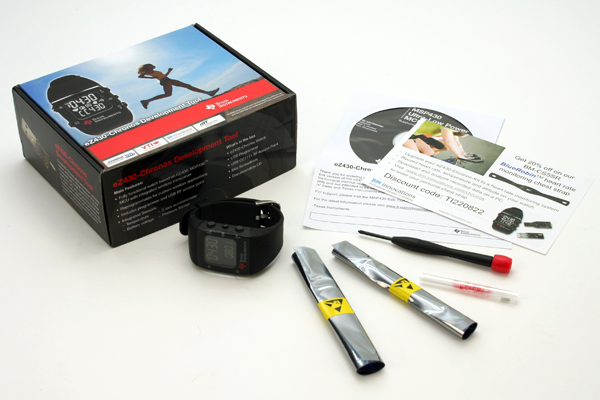
\includegraphics[width=0.7\textwidth]{img/chronos_kit.jpg}
  \caption{Contents of the chronos kit. (Courtesy Marc de
  Vinck)}
  \label{fig:chronos_kit}
\end{figure}

\begin{figure}[h]
  \centering
  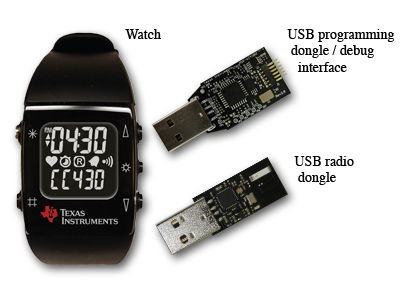
\includegraphics[width=0.6\textwidth]{img/chronos_watch.png}
  \caption{Main elements of the chronos kit. (Courtesy of Texas
  Instruments)}
  \label{fig:chronos_watch}
\end{figure}

\section{Elements of the watch}
A Chronos watch is battery powered and has a typical wrist strap that
allows for wearing it like any other watch. Its uniqueness, however,
comes from what lies within the housing. Of the more common elements
it has a {\bf 96 segment LCD display}, which includes two rows of
digits, respectively 4 and 5 digits long, and many other symbols. All
segments can be lit (and even blinked) independently.  This allows the
watch to display crude letters along with numbers. The available
segments are shown in Figure \ref{fig:chronos_segs}.  The watch also
has 5 programmable buttons, one of which controls the screen
back-light.

\begin{figure}[h]
  \centering
  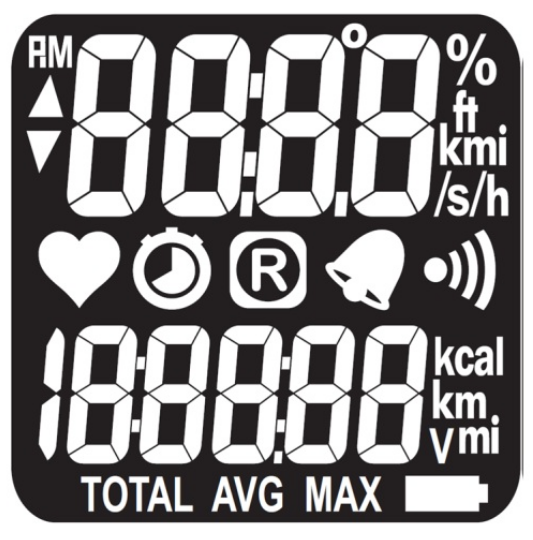
\includegraphics[width=0.4\textwidth]{img/chronos_segs.png}
  \caption{All segments of the LCD display. (Courtesy Texas
  Instruments)}
  \label{fig:chronos_segs}
\end{figure}

What's less common is its MCU ({\bf Mobile Compute Unit}) labeled
CC430F6137,  which can be fully programmed by the user. This MCU is a so
called system-on-chip (or SoC), because it contains a built-in {\bf
radio transceiver}. Conveniently it uses the 868 MHz radio band
for which no license is required.

The MCU will be discussed in more detail in the next section.
Moreover the watch has some on-board sensors: an {\bf accelerometer}
and a {\bf temperature and pressure sensor}. The accelerometer can
detect the watch's position relative to the Earth's gravity, notice a
sudden motion and detect if the watch is falling. The thermometer
simply measures the current air temperature, the pressure though is
precise enough to measure even a 0.3 meter change in altitude, which
is sufficient to detect on which floor of a building the watch is. For
this reason, the pressure sensor is often called an {\bf altimeter}.

Finally, the watch casing is water resistant up to 30 meters and hosts
typical CR2032 batteries, which have a capacity of 225 mAh and provide
a nominal voltage of 3.0 V.

\section{Mobile Compute Unit}

MCU is a Compute Programmable Unit (CPU) designed for extremely
low power usage. The one used in Chronos has the MSP430 (Mixed Signal
microProcessor) architecture, which is particularly suited for low
power applications. It belongs to the TI family of products codenamed
CC430 which features 16-bit, RISC based (Reduced Instruction Set
Computing) CPUs \cite{CC430ds}. The exact chip soldered in the watch
is CC430F6137 and its datasheet describes details specific only to this
particular chip \cite{CC430F6137ds}.

Applications that may be run on the watch are limited by MCU's
resources. The most limiting one is memory. There are two types
of memory available:
\begin{itemize}
  \item {\bf 32KB of flash memory}. This is non-volatile fast-read
    slow-write on-chip memory. It stores code and data. After a reset,
    the MCU jumps to a location (address 0x8000) in this memory and
    starts executing instructions recorded there. Although the 32KB of
    flash may seem little, with modern code-size optimizing compilers,
    quite complex applications are possible. For example, this is just
    enough memory to fit a temperature monitoring application in which
    each node sends out its readings and forwards readings of other
    nodes to a single sink node.
  \item {\bf 4KB of RAM} It is very similar to PC RAM and its
    operation consumes a lot of energy. That's why it's amount is so
    small. 4KB is however just enough to fit the temperature monitoring
    application mentioned above.
\end{itemize}

The MCU clock is scalable and can run at the {\bf maximum frequency of
20 MHz}.  MSP430 RISC instructions are however much simpler than, for
example, x86 ones. To give a feel for this difference, 16 MHz (default
in Chronos) was compared to an Intel Core 2 x86 processor clocked at
2.53 GHz. Loops, similar to those of Floyd-Warshal algorithm, were used
in the simulation:

\begin{lstlisting}[numbers=none, language=Pascal]
    enum { N = 300 };
    uint16_t M[N*2];

    void floydWarshal() {
        uint16_t k, i, j;
        for (k = 0; k < N; k++)
          for (i = 0; i < N; i++)
            for (j = 0; j < N; j++) {
                if(M[i+j] > M[i+k] + M[k+j])
                  M[i+j] = M[i+k] + M[k+j];
            }
    }
\end{lstlisting}

Execution on the watch took 27s while on the PC that was only 40ms.
To make a fair comparison we must scale down the PC clock to 16MHz. If
it were so, the execution would take 6.3 seconds. Thus watch MCU
is over 4 times less efficient due to sole architectural differences.
If we count in the clock speed difference, watch is over 670 times
slower than a PC.

However we can crudely compare power consumption in the same way.
Intel CPU uses around 15W of power, while watch MCU only 11mW. If we
scaled the MCU up to PC clock speed it would only use 1.7W. Thus it is
much more power efficient. Everything depends on where the compromise
is made.

\section{Additional hardware functions}

There are certain functions that, though possible to be implemented in
software, are also easily implementable in hardware. Choosing the
hardware approach saves both execution time and energy. Moreover, some
features can be implemented only with hardware support. Let us discuss
the most important hardware features available in the CC430f6137 MCU
(and many other members of the CC430 family for that matter).

{\bf LPM (Low Power Mode) support} allows an MCU to dynamically switch to
one of several power states.  They are called Active, LPM0, LPM1, etc.
Each successive one consumes less energy by disabling more hardware
functions and peripherals. This mechanism is crucial for lengthening
the battery life. To illustrate how important this is, let us present
some crude battery life estimates:

\begin{itemize}
    \item In Active mode (executing instructions), the watch's battery
      would last for a week (6.8 days).
    \item In LPM0 or LPM1 the battery life would grow to roughly 280 days.
    \item In LPM2 the battery would last around 9 years.
    \item And finally in LPM3 or LPM4 it would last half a decade (52
    years), which is more than the battery's shelf-life.
\end{itemize}
If a battery is to last years, an MCU must spend most of the time in
the lowest power modes.

For this reason, another vital subsystem is {\bf Timer\_A}, which
allows for setting an alarm that will fire (interrupt) after a specific
period of time (on the order of milliseconds) and execute certain
piece of code (an interrupt handler). It would be impossible to use low
power modes without such functionality.

Since Chronos is primarily a watch, {\bf RTC\_A (Real Time Clock)} is
provided. This module provides wall clock and calendar functions. It
is the means for accessing seconds, minutes, hours, days of week, days
of month, months, and years.  Moreover it can also be configured as a
general-purpose counter --- something similar to Timer\_A.

The MCU has 64 pins. Most of them are {\bf IO pins}. They can be
configured to act as an input, output or special function.  In input
mode, they inform of the signal that's connected to them (high or
low). Similarly, in output mode, they can generate a high or low
signal \footnote{If one were tempted to connect input and output pins
to experiment with signal passing, if careless, he could destroy the
MCU.  An output pin produces a maximum of several mA of current. An
input pin would then accept all this current. In effect, such a
connection without a resistor would result in a short circuit {\bf
through the chip}. Using a 2k $\Omega$ resistor can alleviate the
problem.}. Special function mode connects the pin to an internal
hardware component i.e.  the LCD driver.  Also it is possible to be
notified (via interrupt) if the state of an input pin changes.  This
enables, for instance, implementing button drivers.

There are more LCD segments on the display than there are pins on the
chip. Even if there were enough, using so many pins for the LCD would
be wasteful. It's better to spread data over time. In a technique
called multiplexing, the chip selects a group of segments by powering
a control pin and lits the ones within this group. Eight group pins
and eight element pins are enough to drive 64 LCD segments in this
fashion. Groups are changed quickly enough that human doesn't notice
any blinking, which makes it a practical solution.  However
implementing this in software would be wasteful, therefore {\bf LCD\_B}
driver does all this in hardware.

Another vital hardware driver is {\bf USCI (Universal Serial
Communication Interface)}. It can be configured to pose as one of
standardized communication interfaces. Most notably these are SPI
(Serial Peripheral Interface), I$^2$C (Inter-Integrated Circuit) and
UART (Universal Asynchronous Receiver/Transmitter). Though cumbersome,
each one can be implemented in software. However, hardware support
increases performance by an order of magnitude. UART, for example, is
particularly important during development, because it allows for sending
text from watch's MCU to a PC.

An interesting and practical feature of the CC430 family is the
ability to do {\bf port remapping} at runtime. Typically special
functions are hard-connected to certain chip pins. For example UART's
Tx and Rx may be mapped to pins P1.0 and P1.1. If we had two
components that wanted to communicate with the MCU chip via UART, some
external circuitry would be needed to reconnect the pins on demand.
This isn't, however, necessary in the CC430 family, because such
functionality is built-in. Hardware drivers can be reconnected to
arbitrary IO pins without powering down the MCU.

The following two hardware features are related to data integrity and
security. The first one is a {\bf CRC module} that speeds up
calculation of check sums.  MSP430 MCUs are poor in doing certain
types of operations like shifts and using this hardware leads to
considerable speed improvements, especially on large data blocks.

The second one is the {\bf AES128 Accelerator}. Advanced Encryption
Standard 128 is a secure symmetric cipher. Its complicated
encryption and decryption algorithms were implemented in hardware.

Finally, the following three hardware functions ease the interaction
of the MCU with analog circuits.  {\bf REF} is a reference voltage
generator. Some components, like the LCD, require a certain electric
voltage for their operation.  Others perform comparisons of external
voltages to a reference voltage. It is convenient to generate such a
reference voltages without the help from external circuitry.

{\bf Comp\_B} is a voltage comparator. It is a circuit that can
compare two voltages and tell which one is higher. Moreover one of
them can be a reference voltage of a known value. Comparators are used
to interface analog signals to digital circuitry.

And finally {\bf ADC12\_A} is an analog to digital converter
module. Conceptually it's a generalized comparator \footnote{In
fact ADC is implemented using several comparators, with varying
reference voltages.}, because it returns multiple bits of information
instead of one.  An ADC circuit can very quickly measure the value of
some external voltage. Therefore, if you wanted to construct a thermometer
you would connect a thermistor (resistance of which reflects its
temperature) to a reference voltage and measure the resulting
voltage with ADC. From that, temperature would be derived.

There are also some subsystems that support development and in field
operation. The {\bf Watchdog Timer} is a circuit that breaks infinite
loops and other MCU hangs. It needs to be refreshed periodically,
otherwise it will reset the device.

{\bf Bootstrap loader} holds an additional operating system on the
device.  Most notably, it allows for software updates, through the
radio or UART.

\section{Radio transceiver}

In the past radio transceivers typically comprised separate chips. In
our case however such a chip, called CC1101, has been integrated into
the CC430F6137 MCU.  It operates on the unlicensed 868 MHz band
\footnote{However, the European Telecommunications Standards Institute
limits the duty cycle and maximal power output on the 868 MHz band.}.
The module is capable of sending and receiving short packets of
data\footnote{Typically up to 63 bytes long, but through software, it
is possible to support longer packets. Theoretically even $2^{16}$
bytes long.}.  The radio module is usually the most power consuming
component and CC1101 is not an exception. Therefore, it is important
to keep it off as much as possible.

\section{Other devices included in the kit}

For the developer, the most important component is the {\bf USB debug
interface}. It allows for:
\begin{itemize}
  \item Programing the device with a binary image (.hex or .exe file).
  \item Receiving text (printf messages) through UART \footnote{A small
    hardware modification is necessary for that. It's described in
    appendix \ref{appendix:uard_pins}.}.
  \item Connecting to the watch with a debugger. In particular, the
    developer can view the program execution, memory and registers in
    the Eclipse IDE.
\end{itemize}
A connection of the debug interface with the watch is shown in Figure
\ref{fig:chronos_dongle}.

\begin{figure}[h]
  \centering
  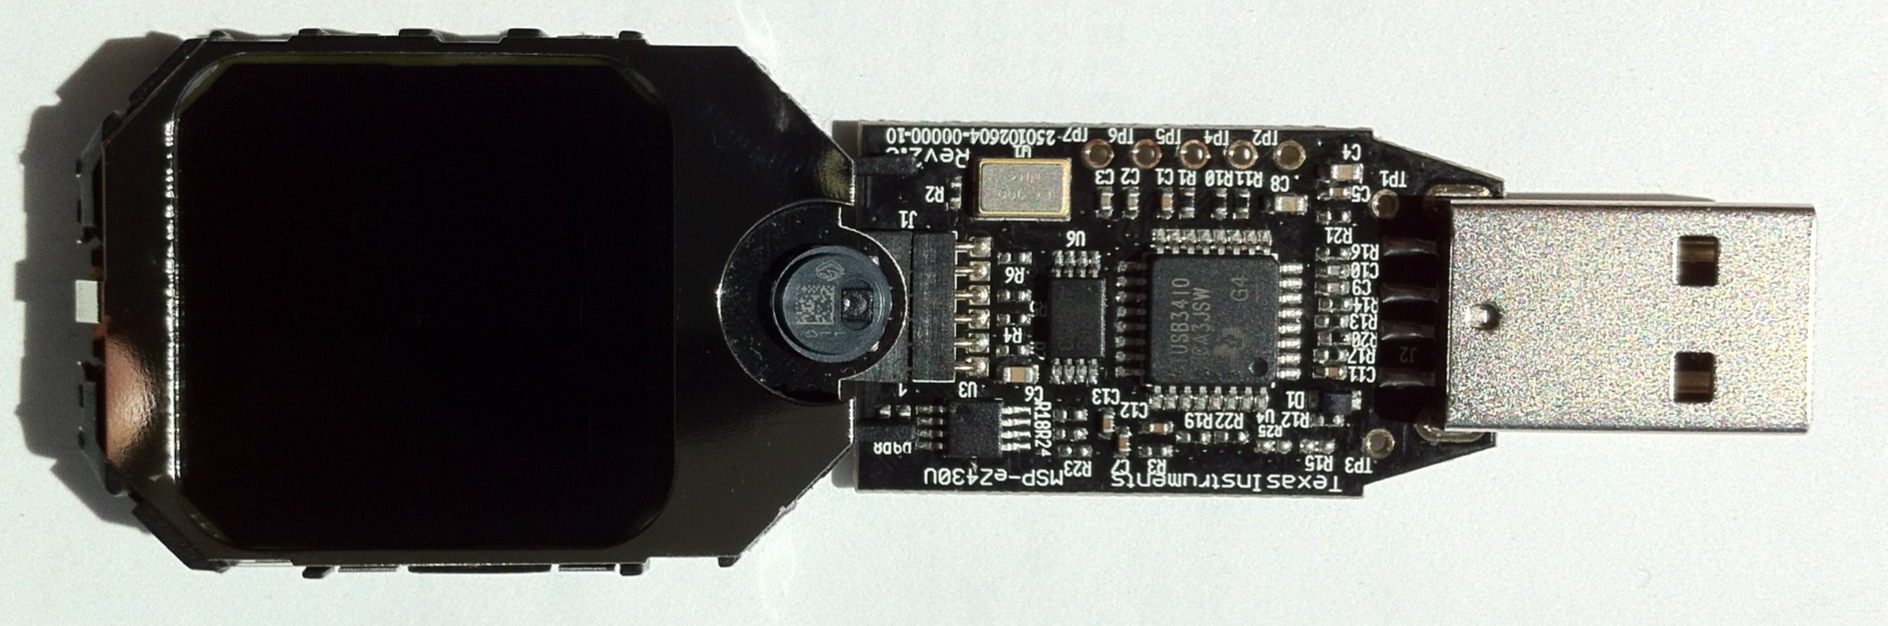
\includegraphics[width=0.8\textwidth]{img/chronos_dongle.jpg}
  \caption{Watch connected to the debug interface.}
  \label{fig:chronos_dongle}
\end{figure}

Another supporting device is the {\bf USB RF access point dongle},
which can communicate with the watch over the radio and also forward
its commands to the PC. One example use is driving a PC mouse by
moving the watch or controlling a presentation with the watch's
buttons. In fact, the dongle also uses a system-on-chip MCU, which
additionally has USB support. Its architecture is, however, different
from MSP430 and currently unsupported by TinyOS. Programming it is an
interesting future work.

The dongle is shown in Figure \ref{fig:chronos_rfdongle}.

\begin{figure}[h]
  \centering
  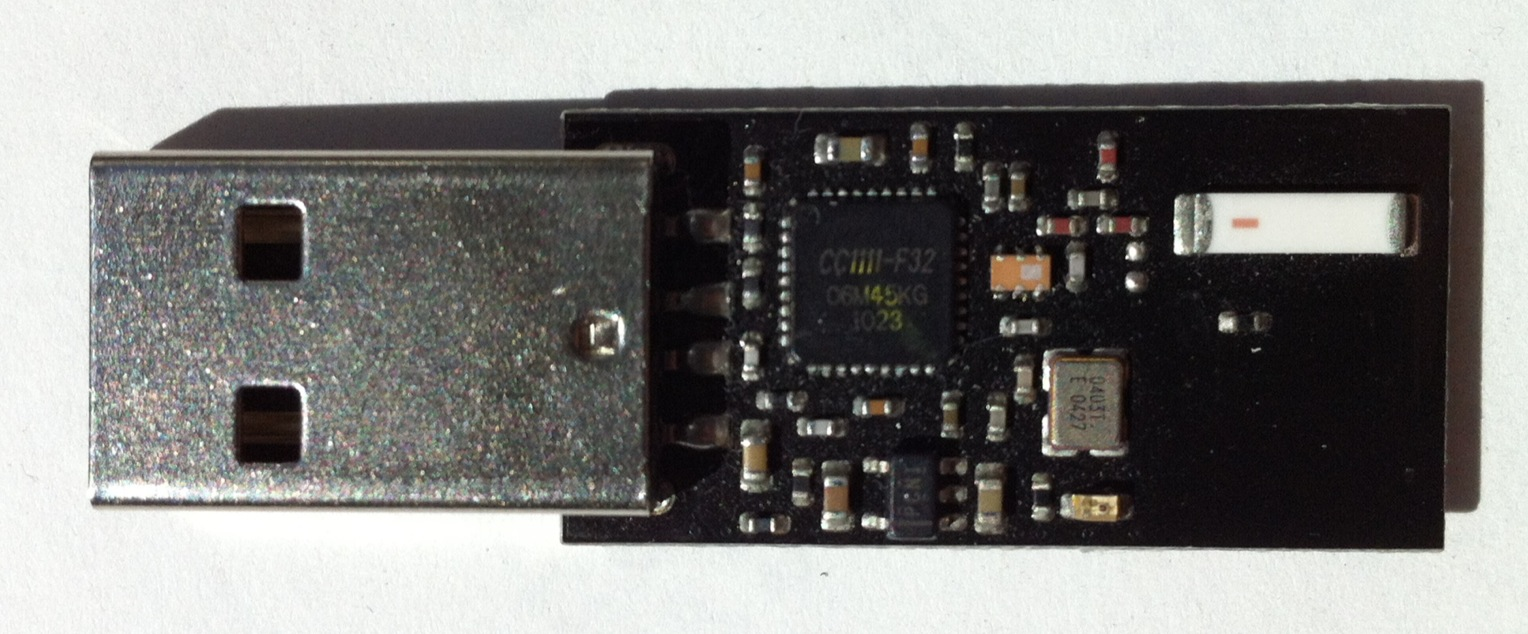
\includegraphics[width=0.6\textwidth]{img/chronos_rfdongle.jpg}
  \caption{USB RF access point dongle.}
  \label{fig:chronos_rfdongle}
\end{figure}

\section{Intended use of the watch}

\subsection{Factory firmware}

Texas Instruments provides software example that is preloaded on every
watch. It provides standard watch functions like time, date, alarm and
stopwatch. Also it shows averaged sensor measurements: altitude,
acceleration, battery voltage and temperature. If an external  heart
rate monitor is present the watch will also display its readings. For
the radio communication, there are few wireless modes:

\begin{itemize}
  \item ACC --- transmit accelerometer motion data.
  \item PPT --- wireless presentation control or bind Chronos
    keys to PC keyboard shortcuts.
  \item Sync --- syncs time and date with PC and calibrates
    temperature and altitude.
\end{itemize}

\subsection{Community use cases}
There are many programs written by technology enthusiasts. Some of the
examples include:

\begin{itemize}
  \item wireless door lock --- a system, of two devices, with which it
    is possible to define a password as a gesture recognized by the
    accelerometer.
  \item flying mouse --- move watch and use it as a PC mouse.
  \item automatic lighting system --- control light bulbs from your
    watch.
  \item Time-based One Time Password (TOTP) Authenticator --- provides
    token based authentication system.
\end{itemize}

\subsection{Shortcomings of existing software}

Applications written for the Chronos watch tend to be simple. Examples
above confirm that. Typically they are written, by one person, to
perform a particular task and share little or no code at all.  While
it would be beneficial if a common software platform emerged from
these efforts, nothing like this happened. Moreover, the
applications listed above, leverage none of the advanced algorithms published in
scientific papers. Chronos watch is, in essence, a mobile wireless
sensor node and not utilizing all the research that has been done on
that field is wasteful. One may expect much more from this platform.

There are three main difficulties that contribute to this situation.
Firstly watch software development is very different from what
developers are used to on the PCs. There is no operating system that
would create abstractions of underlying hardware, like: multitasking,
data persistence, memory protection and process resource management.
Also, inability to run the developed application side by side with
debugging tools makes it more cumbersome to trace problems.  Limited
resources on the MCU, most notably power, require writing more
complicated code - managing the MCU power states being a good example.
Libraries could alleviate that problem, but without a solid software
platform, its difficult to create them. In effect, developer is forced
to write both application and the operating system.

Secondly, the C language it self makes it difficult to manage larger
projects. Basically all names are in a global name space, there are no
boundaries between components and it encourages poor programing
practises, like register bit manipulation without any comments.

Thirdly, working directly with the hardware, creates many new
opportunities for errors. Most common ones are: race conditions during
interrupt handling, memory access violations and leaks, omitted or
doubled component initialization and improper use of hardware.
Moreover in any reasonably complex application there is need for some
form of concurrency.  Implementing it from scratch is difficult and
often causes many additional programming errors.


% Vim settings:
% vim: set textwidth=70:
% vim: set fo+=t:


\chapter{TinyOS and NesC}

\section{The NesC programming language}

Recall traditional C code. In essence it consists of function
definitions and variable declarations listed in some order.  Calling
one function, causes a cascade of other calls, that eventually gets
useful work done. But how to know which function to call? Typically one
would find that out in documentation.

\subsection{Modules and interfaces}

In NesC\footnote{For a deeper discussion of the language see
\cite{NesC}.}, the above issue, is solved more systematically.  Each C code
file must {\bf provide} interfaces, and only through them its
functions may be called. An {\bf interface} is nothing more but a set
of function names that are implemented in the file that provides it.
We call such an interface enriched C file, a {\bf module}.

If interfaces can expose functions to external modules than, by
symmetry, there must also be a way to call functions exposed by those
external modules. To accomplish that, NesC module is not only allowed
to provide interfaces, but can also {\bf use} them. If a module declares to
use an interface, than it's free to call any function this interface
contains. At this point, it isn't however decided where interfaces, it
declares to use, will be implemented. It merely states that it will
need them.

To summarize, a module is a C file that provides a set of interfaces
and uses a different set of interfaces to help it do the work. This
decomposition of an application, that used to be global, into module
sized pieces makes complexity much easier to manage. Moreover,
dependencies between modules are now explicitly declared. To understand
inner workings of a module you only need to see its code and the code
of interfaces it declares to use or provide.

\subsection{Configurations}

We didn't yet mention, how a module that uses an interface, gets
paired with one that provides it. This is done, through a new type of
a file, called a {\bf configuration}. Configurations however, do much
more than just connecting interfaces of modules together.

Firstly, they can use and provide interfaces just as modules
do\footnote{Though only modules contain actual function
implementations.}. In fact, modules and configurations are so similar
than we jointly name them {\bf components}.

Secondly they can instantiate components. By default all components
(modules and configurations) are singletons. If a singleton component
isn't ever instantiated in an application, it's omitted during compilation.

Each configuration first instantiates all components it intends to
work with. Then it defines connections between their interfaces. And
finally, if it has declared to use or provide any interfaces, it passes
these interfaces to components it instantiated.  This means that an
interface provided by a configuration, may be passed through several
layers of configurations until it finally is implemented by some
module.

This mechanism forms basis for creating {\bf self-contained hermetic
abstractions}. Precisely, a top level configuration can provide a set of
useful interfaces and hide all their implementation details. Said
implementation can utilize several layers of abstraction, connect
itself to components shard within application and manage module
initialization, but user doesn't have to know any of it. All he will
have to do, is instantiate this top level configuration in his
application and make use of provided interfaces\footnote{In fact, each
TinyOS application is such a high level configuration, that pulls in
all dependencies and connects them to the module that implements
application logic.}.

We will use graphical representation of components, suggested by
\cite{Bachmaier} (see Figure \ref{fig:example_component}) and, where
it's relevant, we'll distinct modules from configurations by adding
\emph{<<realization>>} or \emph{<<specification>>} stereotypes
respectively.

\begin{figure}[h]
  \centering
  \includegraphics{diagrams/example_component.eps}
  \caption{Component with one provided and one used interface.}
  \label{fig:example_component}
\end{figure}

\subsection{Two-way interfaces}

NesC interfaces are in fact {\bf two-way}. To explain this concept,
we'll consider an example, where user requests an asynchronous
operation. One possible way to support this through interface
connections is shown in Figure \ref{fig:two_way_interface1}. The user
calls \emph{start()} to initiate the operation and provider calls
\emph{completed()} to notify user about it's completion.

\begin{figure}[h]
  \centering
  \includegraphics{diagrams/two_way_interface1.eps}
  \caption{Asynchronous operation implemented with two interfaces.}
  \label{fig:two_way_interface1}
\end{figure}

Though this scheme works, it forces the use of two connections where
there is only one logical association. Need to connect callbacks
separately from requests is an unnecessary nuisance. Instead, NesC allows
{\bf events} to be part of interfaces in addition to normal function
calls known as {\bf commands}. User of such interface will have to
implement handlers for all events, which again are nothing more than C
functions with proper names. Above scheme, implemented using events,
is shown in Figure \ref{fig:two_way_interface2}.

\begin{figure}[h]
  \centering
  \includegraphics{diagrams/two_way_interface2.eps}
  \caption{Asynchronous operation implemented with a two-way interface.}
  \label{fig:two_way_interface2}
\end{figure}

\subsection{Parametrized interfaces}
A component may provide a virtualized resource. This means that a real
resource is split by software to serve several users. For example,
let's consider the problem of waking a group people in a hotel.
Everyone wants to be waken up at different times, but manager only has a
single alarm clock. Solution is simple, he has to set the alarm for
himself, to the nearest waking time of one of his customers. Then, when it
fires, he can wake that person up and reset the alarm to the next
nearest waking time. In essence this scheme crates multiple alarm
clocks using only one. We may say that it virtualizes the alarm clock
\footnote{This is actually a practical problem in low level
programming. Few hardware timers need to be virtualized, to serve
multiple software components.}.

In NesC this would correspond to providing several \emph{Alarm}
interfaces, while using only one. Exactly how many of these virtual
interfaces should be provided, isn't however known ahead of time.
Moreover, if for each virtualized interface, separate function
implementations were needed, it would lead to wasteful code
duplication.

\begin{figure}[h]
  \centering
  \includegraphics[width=1.0\textwidth]{diagrams/parametrized_interface.eps}
  \caption{Parametrized interface used in timer virtualization.}
  \label{fig:parametrized_interface}
\end{figure}

Instead NesC offers {\bf parametrized interfaces}. They differ from
regular interfaces by an additional parameter that their implementing
functions receive. This parameter caries the unique identification
number of the interface that was used to make the call. It can be
treated as a client id.   Notice that this is by far the most
convenient way to implement our alarm replicator, because it can use
this additional argument to index and update an array of firing times
and then easily find the closest one.  Exemplary replication of the
\emph{Alarm} resource is presented in
Figure~\ref{fig:parametrized_interface}
\subsection{Generic components}

Implementing a data structure like \emph{BitVector} as a singleton,
doesn't make much sens. Therefore NesC allows for a component to be
made {\bf generic}. Making a module or configuration generic has two
major consequences.  Firstly all it's instantiations will create
separate and independent components, just as if the code was copied.
Secondly it is possible to pass arguments (both type and value) that
will parametrize such newly created component. Graphically, generic
components are distinguished by the parentheses after their name, as
shown in Figure~\ref{fig:generic_component}. Also note that interfaces
can be type parametrized as well, which greatly supplements generic
components.

\begin{figure}[h]
  \centering
  \includegraphics{diagrams/generic_component.eps}
  \caption{A generic component with type and integer arguments,
  providing a parametrized interface.}
  \label{fig:generic_component}
\end{figure}

\subsection{Memory allocation}
Many errors found on wireless sensor nodes, for which software was
written in C, were caused by various memory related errors. Failed
allocation due to lack of available memory and leaks were problems
particularly painful on nodes with very limited resources.

For this reason, in NesC all memory allocation is static and resolved
during compilation. This way, compiler can easily detect if the
required amount of memory exceeds the amount available on the device.

\section{The TinyOS operating system}

\begin{quotation}
TinyOS is an open source, BSD-licensed operating system designed for
low-power wireless devices, such as those used in sensor networks,
ubiquitous computing, personal area networks, smart buildings, and
smart meters. A worldwide community from academia and industry use,
develop, and support the operating system as well as its associated
tools, averaging 35,000 downloads a year.

It started as a collaboration between the University of
California, Berkeley in co-operation with Intel Research and Crossbow
Technology, and has since grown to be an international consortium, the
TinyOS Alliance.

{\hfill \cite{TOSnet,TOSw}}
\end{quotation}
TinyOS is written in NesC programming language. This means, that its
made of components which interact with each other only through,
separately specified, interfaces. The great advantage of this is
that these components have very clear boundaries and it's easy to
understand how to use them. Consider example\footnote{This isn't a
cleverly chosen example. Components tend to be this intuitive.} shown
in Figure~\ref{fig:platform_serial}.
\begin{figure}[h]
  \centering
  \includegraphics{diagrams/platform_serial.eps}
  \caption{\emph{PlatformSerialC} gives access to the serial port of the 
           Chronos watch.}
  \label{fig:platform_serial}
\end{figure}
It's obvious, that first you need to call \emph{start()}, then send
bytes with \emph{send()} method and optionally call \emph{stop()} when
serial port is no longer needed. Complex details of handling the
hardware are hidden beneath the abstraction.

Another TinyOS's advantage is its portability. Officially it comes
with support for 22 platforms and many more are available through
various project forks. It also comes with many applications that share
its core components, and most of them are platform independent. This
results in a cartesian cross of platforms and applications, which is
incomparably more effective, than having application and platform
tied together.

Testing is also well supported on TinyOS. Firstly, a whole-network
simulator (see \cite{TOSSIM}) is available. It allows to simulate the
software of not one, but a whole network of nodes, on a PC. Moreover
its radio connectivity models are precise enough to draw, reasonably
realistic, conclusions from the simulations. {\bf TOSSIM} is an
invaluable tool for TinyOS developers. Secondly, a NesC unit-testing
framework \cite{TOSMock}, has been recently added to TinyOS. {\bf
TOSMock}'s ability to verify each component's behaviour greatly
supplements high level testing provided by TOSSIM.

Together these advantages make TinyOS, a good platform for scientific
research. It eases the implementation of new algorithms and
techniques.  Richness of already built components, spares the need to
implement everything from scratch.  Also existing components tend to
be better tested, lightening the burden of inevitable programming
errors.  Multitude of supported platforms makes it easy for different
groups to use the same software on their varying hardware.  Comparison
between results is also much easier thanks to the use of a common
system.  Often, researchers can easily run competitive solutions
side-by-site to learn their flaws and find ways to improve on them.
Particularly, in networking research, it's much easier to experiment
with a single element of the network stack, when all the rest of it is
available and tested. It is possible to do incremental improvements
and that is the essence of scientific development.

\subsection{Anatomy of an application}

In this section, we explore a simple TinyOS application and explain
how it works. Its purpose is to periodically blink a
LED\footnote{Light-Emitting Diode}. The root of the application is a
configuration named \emph{BlinkAppC}\footnote{Letter \emph{P}, at the end
of component's name, means that its private, while \emph{C} marks a
useful public abstraction.}. The logic is implemented in module \emph{BlinkC}.
It uses three interfaces to achieve its goals. Firstly, it needs an
entry point. This is provided by the \emph{Boot} interface which sends an
event \emph{booted()} after all system initialization is complete.
Secondly, the LED is controlled through \emph{Leds} interface.
And finally, timing is managed with the help of the
\emph{Timer<TMilli>}\footnote{\emph{TMilli}, is in fact an empty
struct. It serves to distinguish timers with different resolution.}
interface. Whole structure of the application is shown in
Figure~\ref{fig:app_anatomy}.
\begin{figure}[h]
  \centering
  \includegraphics[width=1.01\textwidth]{diagrams/app_anatomy.eps}
  \caption{Structure of the Blink application.}
  \label{fig:app_anatomy}
\end{figure}
The \emph{booted()} event implementation configures the timer to
repeatedly send the \emph{fired()} event.  and its implementation in
turn, toggles the state of the LED.

These interfaces are implemented by three distinct components.
The \emph{LedC} configuration is provided by TinyOS library.
As shown in Figure~\ref{fig:ledc}, it uses a platform specific component
\emph{PlatformLedsC}, which simply gives access to the IO pins to
which LEDs are connected. Most platforms, supported by TinyOS, provide
this component\footnote{Though, some platforms provide fewer leds,
replacing missing ones with stubs. Chronos watch, having no LEDs,
uses it's LCD display.}.
\begin{figure}[h]
  \centering
  \includegraphics[width=0.8\textwidth]{diagrams/ledsc.eps}
  \caption{The \emph{LedsC} configuration. Note that, to use the same
  interface more than once, you have to rename it with the \emph{as}
  keyword.  This can also be done to make implementation more
  self-explanatory.}
  \label{fig:ledc}
\end{figure}

This pattern is quite common. Often platform independent logic is
implemented in the library. To support such library, platform must
implement certain lower level components.  If it doesn't, attempt to
use the library causes a compilation error.

Timer library works this way and is explained, in more detail, in the
next section. \emph{MainC} is related to the system initialization
sequence, therefore task scheduler must be introduced before we look into
it.

\subsection{Timer subsystem}

The generic configuration \emph{TimerMilliC()} serves one purpose. It
provides a single instance of the \emph{Timer<TMilli>} interface and
internally connects it to the component that virtualizes the timers,
thorough a parametrized interface. This way the user doesn't have to
figure out the parameters himself\footnote{Details of how these
parameters are handled, are explained in \cite[ch. 6]{TOSProg}.}.
Figure~\ref{fig:timermillic} shows that the interface is connected to
component \emph{TimerMilliP}.
\begin{figure}[h]
  \centering
  \includegraphics{diagrams/timermillic.eps}
  \caption{The generic \emph{TimerMilliC} configuration.}
  \label{fig:timermillic}
\end{figure}
It is a singleton supporting all instances of \emph{TimerMilliC}. Its
structure is presented in Figure~\ref{fig:timermillip}.
\begin{figure}[h]
  \centering
  \includegraphics{diagrams/timermillip.eps}
  \caption{The singleton \emph{TimerMilliP} configuration.}
  \label{fig:timermillip}
\end{figure}
For the initialization, it relies on the \emph{MainC}
and the timers are actually virtualized by a third component called
\emph{HilTimerMilliC}\footnote{HIL stands for Hardware Independence
Layer. It is explained in section \ref{haa_arch}}. This last one is
provided by the platform, though in its implementation many library
components are used.

\subsection{Tasks and the task scheduler}

Applications need to perform multiple operations simultaneously. As
sensor nodes typically have too little memory to support fully fledged
threads, some other solution is needed. Therefore, NesC cooperates with
TinyOS to provide {\bf task management}. A task, is simply a
parameterless C function with no return value. Tasks are used to split
all lengthy operations into small portions, that can be interleaved
with each other, giving the impression of parallel execution. It's
important to keep the tasks short. Otherwise, throughput of the system
may be reduced, when tasks of several quick operations wait for a
lagging one.

Only one task may runs at any given instant and it can not be
interrupted to run another task. Moreover, a task will only run once
regardless of the number of times that it's posted for execution.
Single bit is preallocated to mark a task as posted.

The execution is handled by the \emph{TinySchedulerC} component,
depicted in Figure~\ref{fig:tinyschedulerc}\footnote{Meaning of the
\emph{async} keyword is explained in Section
\ref{sec:interrupts_and_async}.}. This component is also used by NesC
compiler to generate task related code. Exactly, what happens behind
the scenes, is that when a component declares a task it actually
provides a hidden \emph{TaskBasic} interface. It allows the component
to post task to the scheduler and is obliged to run it, when scheduler
requests it.  All such interfaces are then connected to the
\emph{SchedulerBasicP} module that handles their queueing and also
contains the main task loop.

The \emph{McuSleep} interface is used when the main task loop has been
started but there are no tasks pending. Then MCU enters lowest safe
sleep state\footnote{Sleep level depends on the peripherals left
running. Not all can operate in the lowest power mode.}.

\begin{figure}[h]
  \centering
  \includegraphics[width=1.02\textwidth]{diagrams/tinyschedulerc.eps}
  \caption{The TinyOS's task scheduler structure.}
  \label{fig:tinyschedulerc}
\end{figure}

\subsection{\emph{MainC} configuration and system initialization}

The \emph{MainC} component is special it two ways. Firstly, it
contains the entry point to all TinyOS code, because it implements the
\emph{main()} function. It's characteristic for NesC to, abstract
something like the \emph{main()} function with a component. Secondly,
it handles whole initialization sequence of TinyOS and the current
platform. The diagram of its structure is shown in
Figure~\ref{fig:mainc}.
\begin{figure}[h]
  \centering
  \includegraphics[width=0.98\textwidth]{diagrams/mainc.eps}
  \caption{Structure of \emph{MainC} configuration.}
  \label{fig:mainc}
\end{figure}
The \emph{PlatformC} component is the top level abstraction for the
underlying platform. Its responsibility is to initialize all of the
hardware. This is done, when the \emph{RealMainP}, which contains the
\emph{main()} function implementation, calls the \emph{PlatformInit}
interface. The TinyOS {\bf initialization sequence} consists of the
following steps:
\begin{itemize}
  \item Global function \emph{platform\_bootstrap()} is called to do
    any platform initialization that cannot wait. I.e. disabling the
    watchdog.
  \item Scheduler is initialized through the \emph{Scheduler} interface.
  \item Platform is initialized through the \emph{PlatformInit} interface.
  \item Any tasks requested during platform initialization are ran
    until completion.
  \item Software components are initialized through the
    \emph{SoftwareInit} interface.
  \item Any tasks requested during software initialization are ran
    until completion.
  \item When both hardware and software are ready, hardware interrupts
    are enabled.
  \item \emph{booted()} function of the \emph{Boot} interface is
    called.
  \item Task scheduler enters main task loop.
\end{itemize}
All other software components connect their initialization to
\emph{MainC}. This helps avoid the omitted or double initialization
errors.

\subsection{Interrupt handling and asynchronous events}
\label{sec:interrupts_and_async}

Hardware often needs to notify the software that certain event
occurred. This could be, among others, a radio packet arrival or a temperature
measurement completion. Sending such a notification is possible,
through a mechanism of so called {\bf interrupts}. When an interrupt
condition occurs, processor immediately stops executing instructions
and jumps to a special interrupt handler function\footnote{TinyOS
allows to implement the interrupt handlers with the
\emph{TOSH\_SIGNAL()} macro.}. After it returns, execution resumes
from where it was interrupted.

The fact that interrupts can fire at arbitrary moments causes serious
concurrency problems. They can and often do occur in the middle of
some task being executed.  Consider following scenario: A task is
copying bytes from a queue. Then a radio packet arrives and an interrupt
fires. The handler adds this packet to the queue. But after the task
resumes execution, being unaware of the interrupt, it overwrites queue
state variables with stale values.  Packet is lost and queue ends up
in an invalid state.

Interrupts might be made to wait for the current task to finish.
Alternatively, each interrupt could post a special task to the
scheduler. Neither of these is an option however, because most
interrupts are time critical. For example, if an interrupt notifies
the MCU about a byte received through the serial port, it has to be
handled before the next byte arrives.

NesC and TinyOS solve these concurrency problems by dividing the code
into two parts: synchronous code (SC) and asynchronous code (AC).  All
code reachable from the interrupt handlers is considered to be AC.
Implementation is considered safe, if {\bf each variable is either only
accessed from SC or every access to it is protected with an
\emph{atomic} block}. Tasks, by definition are SC. Commands and
events, that are not SC, have to be marked with the \emph{async}
keyword. In particular, its use shown in
Figure~\ref{fig:tinyschedulerc}, means that tasks can be posted from
AC. Clear separation of the interrupt handling from the normal execution,
reduces the chances of errors and makes code more readable. Moreover, NesC
compiler verifies above constraints and issues warnings, if potential
race conditions are detected. For more information, refer to
\cite[ch. 8]{NesCMan}.

\subsection{The TinyOS component organization structure}

TinyOS components are organized based on their function, hardware
dependence and re-usability. In this section, we list the most
important categories present in the system.

\begin{itemize}
  \item {\bf Global interfaces} are the sews that allow to connect
    many important and independent components. Among them are the
    definitions of \emph{Read}, \emph{Write}, \emph{Send}, \emph{Boot}
    and \emph{Init} interfaces. They are located under
    \emph{tos/interfaces/} path.

  \item {\bf Libraries} contain relatively hardware independent code.
    This means, for instance, that a MAC layer library may assume that
    the radio chip operates on packets, rather than byte streams, but
    it will not assume usage of any particular chip family. Libraries
    are located under \emph{tos/lib/}, \emph{tos/system/} paths. The
    first one, typically contains various protocols and algorithm
    implementations. The second, contains components that are
    integral parts of TinyOS or are heavily shared among platforms.
    Examples include the \emph{LedsC} and \emph{MainC} configurations.

  \item {\bf Chip drivers} contain sets of components, meant to
    operate particular hardware chips. They are located under
    \emph{tos/chips/} path. For example, one of the drivers is called
    \emph{at45db} and supports an external flash memory chip, of the
    same name. Any platform, that makes use of this chip, can also use
    this driver. In hardware design, chips are abstractions that hide
    their internal workings. The same is true about their
    drivers. Often, it's only necessary to make a few component
    connections, that represent physical connections on the circuit
    board, to incorporate the driver into a platform.

  \item {\bf Platforms} contain sets of components needed to support
    particular circuit boards. They are located under
    \emph{tos/platforms/}. One notable example is the \emph{chronos}
    platform, which is the subject of this work. A special file, named
    \emph{.platform}, holds the configuration parameters for the
    compiler. Among others, it lists platform dependencies and the
    MCU the compiler should generate code for. Platform
    directory  also contains the \emph{PlatformC} component, which is
    the main entry point to hardware initialization code, along with
    many other hardware dependent components that enable various
    functions and features.

  \item {\bf Applications} are located under \emph{apps/} path. Each
    consists of a root configuration, helper components, a
    \emph{Makefile} and a \emph{README.txt} file. The \emph{Makefile}
    guides the build process\footnote{It's worth to note, that nowhere
    in an application is any particular platform specified. Instead
    every application can be built for any platform, selected by an
    argument to the \emph{make} command.} and the \emph{README.txt}
    contains useful comments on the application operation.

  \item {\bf Support build rules} are located under
    \emph{support/make/} path. They define exactly how build for each
    platform should progress.

\end{itemize}

\subsection{The Hardware Abstraction Architecture (HAA)}
\label{haa_arch}

Concept of the {\bf Hardware Abstraction Architecture} arises from the
desire, for the hardware related code, to have three valuable
properties. Firstly, we would like the low level code to be clear and
readable. Code that, for example, makes uncommented register accesses
is very difficult to maintain in the long run. Such bad practices also
cause many programming errors, yet they are tempting. Secondly, we
would like to have useful abstractions of all available hardware
features. Often, they allow to make important performance
optimizations. Access to hardware should however be made on a
relatively high level, that prevents errors caused by forgetting
certain details related to it's operation. Such details should be
taken care of behind the scenes. Thirdly, we would like to have
certain abstractions that are hardware independent. Most notable
example is the radio networking, where we want an interface that
allows us to communicate, regardless of the used radio chip. Often
conforming to such interface requires implementing some of its
functions in software, while ignoring some other features that the
hardware provides.

To meet these goals \cite{TEP2}\footnote{TinyOS Extension Proposal}
proposes splitting the code according to a three layer architecture,
handsomely depicted in Figure~\ref{fig:haa_diagram}.
\begin{figure}[h]
  \linespread{0}
  \begin{verbatim}
                           +-----------------------------+
                           |                             |
                           | Cross-platform applications |
                           |                             |
                           +--------------+--------------+
 +-----------------+                      |                  +-----------------+
 |Platform-specific|                      |                  |Platform-specific|
 |  applications   |                      |                  |  applications   |
 +--------+--------+                      |                  +--------+--------+
          |          Platform-independent | hardware interface        |
          |        +-------------+--------+----+-------------+        |
          |        |             |             |             |        |
          |  +-----+-----+ +-----+-----+ +-----+-----+ +-----+-----+  |
          |  |.----+----.| |.----+----.| |.----+----.| |.----+----.|  |
          |  ||         || ||         || ||         || ||  HIL 4  ||  |
          |  ||  HIL 1  || ||  HIL 2  || ||  HIL 3  || |`----+----'|  |
          |  ||         || |`----+----'| |`----+----'| |     |     |  |
          |  |`----+----'| |     |     | |     |     | |     |  +--+--+
          +--+--+  |     | |.----+----.| |     |     | |     |  |  |
             |  |  |     | ||         || |.----+----.| |.----+--+-.|
             |.-+--+----.| ||         || ||         || ||         ||
             ||         || ||  HAL 2  || ||         || ||         ||
             ||         || ||         || ||  HAL 3  || ||  HAL 4  ||
             ||  HAL 1  || |`----+----'| ||         || ||         ||
             ||         || |     |     | ||         || ||         ||
             ||         || |     |     | |`----+----'| |`----+----'|
             |`----+----'| |.----+----.| |     |     | |     |     |
             |     |     | ||         || |.----+----.| |     |     |
             |.----+----.| ||  HPL 2  || ||         || |.----+----.|
             ||  HPL 1  || ||         || ||  HPL 3  || ||  HPL 4  ||
             |`----+----'| |`----+----'| |`----+----'| |`----+----'|
             +-----+-----+ +-----+-----+ +-----+-----+ +-----+-----+  HW/SW
                   |             |             |             |          boundary
        ************************************************************************
            +------+-----+ +-----+-----+ +-----+-----+ +-----+-----+
            |HW Plat 1   | |HW Plat 2  | |HW Plat 3  | |HW Plat 4  |
            +------------+ +-----------+ +-----------+ +-----------+
  \end{verbatim}
  \centering
  \caption{The Hardware Abstraction Architecture (source \cite{TEP2}).}
  \label{fig:haa_diagram}
\end{figure}
Each layer is founded on top of the previous one, hardware being at
the bottom and hardware independent applications at the top. Now we'll
describe purpose and function of each of the HAA layers.

Right above the hardware lies the {\bf Hardware Presentation Layer
(HPL)}. Its purpose is to hide, often crude, ways in which hardware is
accessed behind NesC interfaces. It's possible for several
components to form the HPL layer. For example, register access can
better handled if register reading and writing is separated from
meaning of these operations. But these components should have no
state, no logic and only precisely present commands that can be sent
to the hardware and translate interrupts that it fires into
asynchronous events. The rationale for this, is that we want to keep
HPL components as simple as possible, because hardware access makes
them already complex enough.

The {\bf Hardware Abstraction Layer} is made of components that
implement all the logic to handle the hardware. They access it through
HPL and provide abstract, easy to use interfaces for application and
the HIL layer. HAL can have state and should use it to hide the burden
and subtleties related to hardware operation. On one hand it should
ease the application development and on the other allow to fully
utilise the hardware, for maximum application performance.

By its nature, HAL is hardware dependent. Therefore, on top of it,
the {\bf Hardware Independence Layer} is introduced. It should provide
a set of well defined\footnote{Most HIL interfaces are described in
TEPs.} interfaces, which in their design, are balanced for hardware
independence. Often there is a discrepancy between hardware features
and what is required to meet the interface.  Designers try to shorten
this gap by distilling a common subset of functions typically
available in most types of hardware. Still there may be need to either
virtualize the resource or provide some kind of access arbitration to
hide its singleton character and provide other features through
software algorithms.

Typically, developer should first try to use only HIL interfaces in
his application and only, if considerable performance gains are possible,
should he resort to using the HAL interfaces. This way, maximum
hardware independence is assured.

\subsection{Integrated power management and concurrency control}

Power management is critical in sensor network applications, which
rely on batteries. One aspect of this is related to peripheral devices
- external chips, MCU subsystems and data buses. They need to be
powered down whenever they are not in use\footnote{Actually, the best
policy is to power devices down when they are not in use for a specific
period of time.}. For this, exact information about the device usage
is needed.  Getting it is tricky however, because multiple clients may
compete for access to the device and it has to be arbitrated, to avoid
collisions.  This leads to the conclusion, that joining concurrency
control and power management may be beneficial. Knowing the
concurrency, we can share the device among clients and also power it
down when its not in use.

\cite{Klues et al.} proposes an elegant design that allows to
implement this idea in TinyOS. We will present it on the following
example, which closely resembles real applications:

Assume that the node contains a certain hardware device. This
device can perform several functions, but only one can be selected at
a time and only one user can use the device at any time. Moreover, it
is necessary to power down the device once its current function has
been deactivated. There are several clients wishing to use the device
and each knows ahead of time which function it's interested in.
\begin{figure}[h]
  \centering
  \includegraphics[width=1.0\textwidth]{diagrams/devicearbiterp.eps}
  \caption{Component that arbitrates access to the device and powers
  it down when not in use.}
  \label{fig:devicearbiterp}
\end{figure}

Solution consists of two abstractions. Arbitration between the clients
is handled by the \emph{DeviceArbiterP}, which uses a system library
component named \emph{FcfsArbiterC}. The first-come-first-server
arbiter queues requests for device access and grants it to each client
in turn. It also takes care of configuring the device for each client,
before granting the access. Finally, when there are no more pending
requests, it leaves the device to its default owner - the
\emph{DevicePowerDownP}. This power manager, turns the device off upon
acquisition and  on when it's requested again by the arbiter.
The connections, are shown in Figure~\ref{fig:devicearbiterp}. Users do
not access \emph{DeviceArbiterP} directly though, but rather use a series of
generic function access components. One of them is shown in
Figure~\ref{fig:devicefunction1}.
\begin{figure}[h]
  \centering
  \includegraphics[width=1.0\textwidth]{diagrams/devicefunction1c.eps}
  \caption{Generic configuration that client uses to access the
  the device.}
  \label{fig:devicefunction1}
\end{figure}
A client wanting to use the first function of the device creates an
instance of this configuration, which gives him \emph{Resource} and
\emph{DeviceFunction1} interfaces. The first one must be used to
secure access to the device.  Then, second one allows to actually use
the device.  Note that, in NesC it's possible to wire twice to the
same interface.  \emph{DeviceFunction1P} uses this feature, to assert
that device access really was acquired by the user. In a variation of
this schema, it could acquire the resource behind the scenes as well.

% Vim settings:
% vim: set textwidth=70:
% vim: set fo+=t:


\chapter{Porting TinyOS for Chronos hardware}

This chapter describes the work done to make TinyOS run on Chronos watch. Firstly, we show how we added a minimal, yet functional, platform to the OS. Then, we discuss the methodology used for introducing new code and go over a basic MCU configuration, which is fundamental for the operation of other systems. Afterwards, we present a conceptual schema of the watch circuits that, most notably, shows connections between the hardware components. The remainder part of the chapter describes the hardware drivers we have created, starting with the MCU internal systems and going towards the peripherals.

\section{Adding a minimal functional platform}

The first milestone of our project, was to get to the point, where we could compile the \emph{Null} application and upload its image to the watch. Although this application is of little use, it does basic system initialization. Therefore, it allows for verifying the build configuration. The additional benefit was that we could learn the TinyOS build process.

To compile code for the MSP430 architecture, we used \emph{\bf msp430-gcc}. This was an obvious choice, because the NesC compiler has a built-in support for \emph{gcc}. Its installation wasn't, however, as easy as one might expect. Namely packages provided in Ubuntu were too old and did not contain headers for the \emph{CC430F6137} MCU. In the end, we removed all related system packages and built \emph{msp430-gcc} from sources, using the most recent version available at the time: 4.6.2.  In addition to the compiler, tools like \emph{msp430-gdb} and \emph{mspdebug} were also installed.

The \emph{\bf mspdebug} tool is particularly important for Chronos development, as it allows for flashing software on the watch through the USB debug dongle.  Additionally, it allows for debugging code running on the watch: it provides a primitive gdb server, to which \emph{msp430-gdb} is able to connect\footnote{It's imperative to use the most recent version of \emph{msp430-gdb}, because older versions are not compatible with the \emph{mspdebug} tool.}.

Afterwards, the {\bf NesC compiler} was installed from sources as well. Then we choose and installed a clean upstream version of the TinyOS, provided by \cite{TOSnet}. It contained some tools and scripts and we installed those too.

At that point, we had a functional TinyOS installation, capable of targeting MSP430-based boards, like \emph{telosb}. We choose to name the new platform for our watch as \emph{chronos}. To make if fully functional, we had to create a few files under the \emph{tos/platforms/chronos} path, among which only \emph{.platform} was non-trivial. This configuration file holds various compilation parameters, in particular, the exact MCU model used in the watch, so that the generated binary images get correct offsets for the code segment (0x8000) and the interrupt vector (0xFF80).

We also wanted the build process of an application to be initiated with a standard TinyOS make command:
\begin{lstlisting}[numbers=none, language=bash]
  $ make chronos install
\end{lstlisting}
For this to work, we had to add a configuration file under the \emph{tos/support/make} path. The \emph{chronos.target} file adds our platform to the build system, which in turn takes care of the exact NesC compiler invocations. In addition, file \emph{mspdebug.extra} was added under the \emph{tos/support/make/msp} path, which invokes the commands that program Chronos.

These changes may seem obvious, but it took us quite some time to work them out. Eventually, we reached a point where the \emph{Null} application was successfully installed on the watch.

\section{Code creation methodology}

The next step was to add code that would make the watch operational. Generally it's considered a good programming practice to reuse existing code rather than write it from scratch. Existing code tends to be more tested and can save considerable time, especially when it contains nontrivial constructions that would otherwise require a test and debug cycle to discover. Such situations are especially frequent when dealing with hardware. Moreover, our project was quite time constrained from the beginning and various delays were to be expected further on. Under those circumstances, saving time wherever possible was particularly important. We benefited greatly from the fact that TinyOS code licensing is very liberal, allowing for free use, with few reasonable restrictions, like preserving the license headers in files.

Nevertheless, not all goals could be completed by adapting existing components. In cases where no drivers in NesC were available, we had to fall back to the hardware documentation in the form of datasheets. They describe hardware's behaviour well, though sometimes certain issues were only discovered and compensated for after the driver code was implemented and run. As a rule, documentation is low level, describing only control registers available on the device. All higher-layer  abstraction had to be devised and implemented by us. This was a tedious task and applying the Hardware Abstraction Architecture eased it enormously. We didn't know that from the beginning, though. Therefore, some designs follow it better than others. Besides, in practice boundaries between layers aren't always clear.

A few times we encountered code that was close to what we needed, but some hardware differences precluded using it directly. Modifications had to be done before it could be added to the Chronos platform. In those cases, we had to mix the above approaches by studying the datasheets to understand the inner workings of the code. However, we found that both contributed to better understanding. Code told us much about the inner workings of the hardware and datasheets helped understanding the constructions used in the code. Most notably, such an approach was used to port the low level radio driver, but the principle extends to other components. As a rule, it was much easier to understand the operation of a hardware device if, even a crude, driver implementation was available.

To implement the code, we first used traditional terminal based tools, like the \emph{vim} editor. Later on, when we discovered the \emph{Yetti 2} plugin (see Appendix \ref{ch:prog_env}), we started using \emph{Eclipse} with all its benefits. This increased our productivity considerably. Moreover, there is no emulator of the watch available. Therefore, all testing had to be done by uploading images to the hardware and observing its responses. At first, we didn't even know if programming was successful, but when the LCD display became available, followed by the serial console, and ultimately visual debugger, the process became quite seamless. See Appendix \ref{ch:prog_env} for details.

Finally, in what we believe is \emph{the way} to create code for mobile platforms, we tried to use \emph{TOSMOCK} for module unit-testing. This technology, however, became available too late to be widely used in our code.

\section{MCU configuration}

The MCU configuration was made much easier, thanks to the existence of a partial port of TinyOS to a similar hardware platform. The Texas Instruments \cite{EM430}, shown in Figure~\ref{fig:em430_board}, is a development board which uses the exact same \emph{CC430F6137} MCU chip as Chronos does. Work on the port was done as a part of the \cite{OSIAN} project. Even though Chronos and EM430 differ in peripherals, much of the internal MCU configuration code was compatible and we decided to reuse it.  Minor modifications were required to meet our coding standards and, to fix a few issues.
\begin{figure}[h]
  \centering
  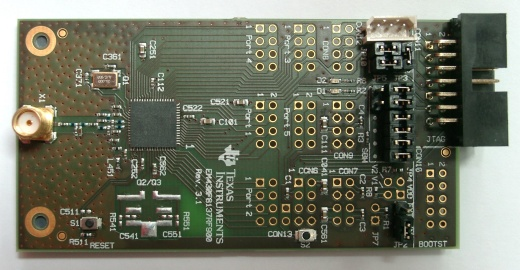
\includegraphics[width=0.7\textwidth]{img/em430_board.jpg}
  \caption{The Texas Instruments EM430F6137RF900.}
  \label{fig:em430_board}
\end{figure}

The entire MCU configuration is done in the \emph{PlatformC} and \emph{PlatformP} components, shown in Figure~\ref{fig:platformc}.
\begin{figure}[h]
  \centering
  \includegraphics[width=1.0\textwidth]{diagrams/platformc.eps}
  \caption{\emph{PlatformC} performs MCU initialization.}
  \label{fig:platformc}
\end{figure}
The first step that \emph{PlatformP} takes is disabling the watchdog timer. Otherwise, the timer would shortly reset the device. Disabling the timer requires only a single register assignment and is done inline. In the future, we may wish to use the watchdog to increase Chronos's reliability, but it wasn't a priority in this stage of the project.

One of the primary MCU responsibilities is providing clocks and timing for other subsystems. Let's first look at timers. In Section \ref{ch:timer_subsystem}, we introduced TinyOS timer library stating that \emph{HilTimerMilliC} is provided by each platform. Continuing that discussion, Figure~\ref{fig:hil_timer_milli_c} shows a simplified structure of this component, as it is provided by the \emph{chronos} platform.
Let's explain its operation in a bottom-up order.
\begin{figure}[h!]
  \centering
  \includegraphics[width=0.55\textwidth]{diagrams/hil_timer_milli_c.eps}
  \caption{Structure of Chronos's \emph{HilTimerMilliC}. (simplified)}
  \label{fig:hil_timer_milli_c}
\end{figure}

The \emph{Msp430Timer32khzC} gives access to one of the hardware timers. \emph{Msp430AlarmC} uses it to provide an \emph{Alarm} interface with a 32kHz granularity and a 16-bit range. Then, it is transformed by \emph{TransformAlarmC} into a wider 32 bit alarm with 1ms (actually $10^6 / 2^{10} \approx 976.5\upmu$s) granularity. Finally, this alarm is converted into a timer and virtualized. Note that these transforming components all come from the TinyOS library.

The millisecond granularity isn't, however, sufficient for some of the Chronos peripheral drivers. Where delays on the order of microseconds are needed we didn't want to resort to active waiting. Having latency and memory footprint in mind, we decided to implement virtualized 16-bit microsecond alarms\footnote{Note, that microsecond timing is quite imprecise. Firstly it's difficult to get an event fired within 10$\upmu$s and the exact firing time can vary by as much as 25$\upmu$s. Still, if a 37$\upmu$s delay is necessary, a microsecond alarm is the best choice.} in addition to millisecond timers. They are more light-weight than timers. Therefore, we can use them more liberally. The alarm structure is shown in Figure~\ref{fig:virutal_alarm_micro_16_c}, and its operation is similar to the timers described above.
\begin{figure}[h]
  \centering
  \includegraphics[width=0.55\textwidth]{diagrams/virutal_alarm_micro_16_c.eps}
  \caption{Structure of \emph{VirtualAlarmMicro16C} generic component.}
  \label{fig:virutal_alarm_micro_16_c}
\end{figure}

The MSP430 specific timer code comes from \emph{tos/chips/msp430/timer} library. However, for the CC430 MCUs, the HPL layer has been overwritten with the \emph{tos/chips/msp430/msp430xv2/timer} components, which we've taken from the EM430 port.

The \emph{Msp430Timer32khzC} and  \emph{Msp430TimerMicroC} components, used above, provide access to 16-bit hardware counters Timer\_A0 and Timer\_A1, running at 32kHz and 1MHz respectively. They are implemented in this new HPL layer, but their structure is relatively simple and mundane so we will omit it. For details, see the mentioned libraries.

Let's nos describe the configuration of Chronos clocks, which generate driving signals for timers and other subsystems. There are three major clocks available on the platform. The first is the {\bf REFOSC}, which uses an internal 32kHz oscillator. The second is the {\bf DCO} that uses an internal high-frequency digitally-controlled oscillator, which we run at 32MHz. The third is the {\bf XT1}, powered by an external 32kHz crystal oscillator. This last one supports very low power operation: the MCU can be left in deep sleep state, while the external oscillator drives the clock that can then wake it up. In this mode, only a tiny current is consumed. We didn't, however, utilize this option leaving it for future research.

The MCU subsystems are actually fed from so-called clock sources. This indirection allows for modifying the clock signal before passing it on. In particular, it allows to scale down the frequency by a constant factor. There are three clock sources in CC430 MCUs. The {\bf Master Clock (MCLK)} that drives instruction execution, the {\bf Sub-System Master Clock (SMCLK)} that drives MCU peripherals, and finally, the {\bf Auxiliary Clock (ACLK)} that drives subsystems where slower frequencies are needed.

Clock configuration is done by the \emph{Msp430XV2ClockC} component, which is part of the \emph{tos/chips/msp430/msp430xv2/timer} library. Its structure is presented in Figure~\ref{fig:Msp430XV2ClockC}.
\begin{figure}[h]
  \centering
  \includegraphics[width=0.95\textwidth]{diagrams/Msp430XV2ClockC.eps}
  \caption{The clock configuring component.}
  \label{fig:Msp430XV2ClockC}
\end{figure}
The \emph{Msp430XV2ClockP} module configures all the clocks during its initialization. It does it through the \emph{Msp430XV2ClockControl} interface which is also made available externally, so that applications can tune the configuration if needed. Note that the default MCU instruction execution speed can be modified in \emph{Msp430XV2ClockP}. This is possible through changing the DCO frequency. \emph{Msp430XV2ClockControlP} will set MCLK to half of the DCO speed, but it will always set SMCLK to 1MHz\footnote{This is one of the reasons why we drive Chronos MCU at 16MHz rather then maximum 20MHz. It is not possible to scale DCO from 40MHz to 1MHz to drive SMCLK.} and ACLK to 32kHz. Many subsystems depend on these clock sources having constant and known values. In particular, the above module, also sets the Timer\_A0 to use the ACLK and Timer\_A1 to use the SMCLK. Moreover USCI uses SMCLK to drive UART, SPI and I$^2$C buses. These settings are summarised in Table \ref{fig:clock_speeds}.
The \emph{Msp430XV2ClockControlP} needs to cooperate with \emph{McuSleepC}, because of a hardware flaw present in the CC430F6137 MCUs. The workaround code needs to be notified about the MCU going to sleep and waking up to calculate the sleep period length and also to control the lowest sleep state that can be used.
\begin{table}
  \centering
  \begin{tabular}{ | l | l | }
    \hline
    Subsystem & Used frequency \\
    \hline
    DCO & 2MHz, 4MHz, \ldots, 32MHz \\
    REFOSC & 32kHz \\
    MCLK & DCO / 2 \\
    SMCLK & DCO scaled to 1MHz  \\
    ACLK & REFOSC \\
    Timer\_A0 & ACLK \\
    Timer\_A1 & SMCLK \\
    UART, SPI and I$^2$C & SMCLK \\
    \hline
  \end{tabular}
  \caption{Clock frequency convention used in Chronos.}
  \label{fig:clock_speeds}
\end{table}

The last action taken by the \emph{PlatformC} component is the configuration of \emph{Power Management Module}. This subsystem controls the voltage fed to the MCU logic core and it needs to be increased if higher MCLK frequency is used. At lower frequencies, power can be conserved by reducing this voltage, however, setting it too low may cause unexpected behaviour. PMM can be set to one of four levels, starting with 0. The radio core can only operate at levels 2 and 3. 16MHz MCLK is also the highest frequency that can be used on PMM level 2. Therefore, we decided that it will be optimal to set it to 2.

It's worth noting, that we only noticed that PMM needs configuration after examining the EM430 code. That implementation, however, wasn't correct, because the datasheet explicitly forbids changing the PMM level by more that one step at a time. We've corrected this in our implementation.

\section{Overview of the watch's subsystems}

In this section we present a high level schema of the Chronos systems. The Figure~\ref{fig:chronos_schema} gives a 
\begin{figure}[h]
  \centering
  \includegraphics[width=1.05\textwidth]{diagrams/chronos_schema.eps}
  \caption{Overview of Chronos subsystems and circuit board}
  \label{fig:chronos_schema}
\end{figure}
practical overview of the platform structure. The central rectangle defines the boundaries of the MCU. Beyond it, lie the external components. The connections between them, roughly present the number of wires used and more importantly, what protocol does the communication conform to. Recall that UART is the Universal Asynchronous Receiver/Transmitter and is typically used to communicate with the PC; SPI is the Serial Peripheral Interface and is used to communicate with more advanced external chips; I$^2$C (aka. I2C) is the Inter-Integrated Circuit bus used to communicate with simpler devices, like thermometers. IO, in turn, means that the interaction is done by simply setting lines to high or low states, without using any specific communication protocol. Finally, LCD segment serialization was described in Section \ref{ch:hardware_functions}. Rectangles with bold font captions name hardware subsystem, while those with regular ones denote software components.

Rather than give brief descriptions of each of the seven major component groups presented in the schema, and then repeat the same information in the discussion of driver code, we'll end here and refer to the schema from later sections.

\section{Chronos hardware drivers}

Below we describe the code that was created to make the peripherals of Chronos watch operational. We go through the structure of the software of all major elements of the \emph{chronos} platform, while also making notes on some of the difficulties we encountered during our work.

\subsection{LCD display}
Gaining access to the watch's LCD display was a vitally important step on the path to making Chronos operational.  Before that we had no way of checking if our software is actually running. There are no LEDs on the watch's circuit board, which could normally be used to send first bits of information from the device. We did have the \emph{mspdebug} tool and the USB debug dongle, which together are capable of controlling code execution. However, reasoning anything from raw debug server data proved difficult. Fortunately, a careful study of documentation was enough to blindly configure the LCD\_B subsystem and, with a bit of luck and some hours of restudying the datasheet, we managed to activate the LCD display. Then, we were gradually enhancing the driver, while progress on the rest of the project was made, until it became fully functional. In particular, it even gained the ability to display short text strings.

\begin{figure}[h]
  \centering
  \includegraphics[width=0.8\textwidth]{diagrams/platform_lcd_c.eps}
  \caption{Structure of the LCD display driver.}
  \label{fig:platformc_lcd_c}
\end{figure}
Let's now describe the LCD driver's implementation. The top-level component for the LCD driver is \emph{PlatformLCDC} shown in Figure~\ref{fig:platformc_lcd_c}.
Hardware configuration of the refresh frequency, multiplexing, IO pin special functions, voltage control pump, internal biasing, display memory and internal voltage generation all happens in the \emph{HplCC430LCDBP} module. The module provides a simple \emph{StdControl} interface to turn these settings on and off. The actual display control is implemented in \emph{LCDDriverC}, which provides the \emph{LCDDriver} interface. It is the only interface that an application user cares about. It is also presented in Figure~\ref{fig:chronos_schema}.

On top of the LCD driver, the \emph{PlatformLedsC} component is built. Its structure is presented in Figure~\ref{fig:platform_leds_c}.
\begin{figure}[h]
  \centering
  \includegraphics[width=0.75\textwidth]{diagrams/platform_leds_c.eps}
  \caption{Structure of chronos abstract LEDs provider.}
  \label{fig:platform_leds_c}
\end{figure}
The TinyOS libraries expect that it will provide three \emph{GeneralIO} interfaces for the LEDs and take care of their initialization. \emph{LCDIconIO} generic module, adapts a specified LCD icon to the \emph{GeneralIO} interface. This an example of the TinyOS Adapter design pattern, more information on which can be found in \cite[ch. 8]{TOSProg}.

Finally note that the LCD driver is a poor example of applying HAA. However, due to its simplicity we decided that this is acceptable.

\subsection{Button support}

Buttons enable user input. They are, however, one of these things that sound simple to implement, but are not. A major problem lies in a phenomenon called bouncing, which happens when a button is pressed. The metal contact isn't immediate, causing signal fluctuations preceding the state transition. Figure~\ref{fig:bouncing} illustrates this phenomenon.

\begin{figure}[h]
  \centering
  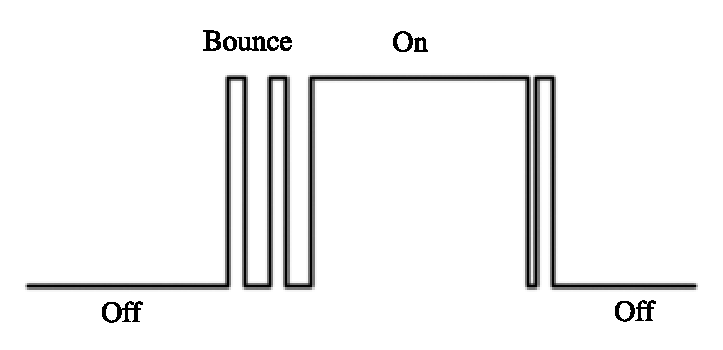
\includegraphics[width=0.45\textwidth]{img/Bounce.eps}
  \caption{Bounce effect in buttons.}
  \label{fig:bouncing}
\end{figure}
The fluctuations may cause several false press and release events. To solve this problem, so-called de-bouncing is applied. This technique, measures the state of the signal several times, with each measurement separated by a short delay. A button press event is only generated if all measurements confirm that the button is pressed.

The algorithm implemented in the generic component \emph{DebouncedButtonC} waits for an interrupt, which notifies about a button state change, and then, probes three more times during a 60ms interval. All edge cases were taken care of. This includes false alarms, when after the interrupt, the state doesn't seem to be changed or when the state changes just before we rearm the interrupt.

This component was made generic, because Chronos has five buttons. In Figure~\ref{fig:UpButtonC} we present the structure of one of them. All others are supported in the same way.

\begin{figure}[h]
  \centering
  \includegraphics[width=0.85\textwidth]{diagrams/UpButtonC.eps}
  \caption{The \emph{UpButtonC} abstraction.}
  \label{fig:UpButtonC}
\end{figure}
The \emph{HplMsp430GeneralIOC} and the \emph{HplMsp430InterruptC} are TinyOS library components that give access to GIO pins for MSP430 MCUs. The first provides access to pin state control, which allows for setting or probing the value of a pin. The second allows for arming interrupts that fire when the state of a pin changes. This is used to discover when a button is pressed.

An application using a button can either check the button's state with the \emph{Get} interface or be notified about a change through the \emph{Notify} interface. Finally note that thanks to the independency of the button implementations, it is possible to recognize press combinations.

\subsection{Buzzer}

Chronos has a built-in sound emitting device, called the buzzer. It can emit beeps typical to alarm clocks.

The buzzer isn't connected directly to an IO pin, as Figure~\ref{fig:chronos_schema} would suggest. Instead, an IO pin triggers a transistor that closes the buzzer's circuit. A 47k$\Omega$ resistor ensures that only a minimal current is drawn from the MCU. Drawing large currents from IO pins is not recommended and can be harmful.

The IO pin needs to be set high, to close the buzzer's circuit, which, in turn, moves its membrane one way. Cutting the current moves the membrane back. This way, a rectangular signal from the IO pin is transformed into sonic waves. The frequency of the waves is the same as the frequency of the signal.

We started the driver implementation by trying to actively generate this rectangular wave. Interestingly, we found that the resulting beeps had artifacts. The tone wasn't clear. As it turned out, after disabling the interrupts the artifacts disappeared. What we heard, were interrupts firing and interleaving with the signal. This is the first time that we've been able to observe interrupts using human senses!

Even though active signal generation with interrupts disabled is hardly a good solution, we had neither need nor time to investigate other options. Therefore, we left the improvement of the implementation for future work. The root component of the buzzer driver is \emph{BeeperC}, depicted in Figure~\ref{fig:buzzer_c}.
\begin{figure}[h]
  \centering
  \includegraphics{diagrams/buzzer_c.eps}
  \caption{The buzzer driver structure.}
  \label{fig:buzzer_c}
\end{figure}
It uses \emph{BusyMicroWaitC} to generate a wave form. This is more wasteful than setting an alarm, but also much more precise, and precision is necessary to generate a clear tone. \emph{BeeperC} provides a simple interface that enables sounding a single beep or a whole \emph{Power Rangers} style hail signal\footnote{It is used in the Zordon demo application.}. Though this hail is long, interrupts are only disabled while each distinct sound is emitted. This allows for processing all pending interrupts between the sounds.

The support for the Buzzer, the LCD display, and the buttons allow Chronos to be a standard hand watch. Let's now discuss more advanced features that distinguish it form such devices.

\subsection{The CC1101-based radio module}

The CC1101 is a radio transceiver chip made by Texas Instruments. Among others, it is used in the SOWNet's \cite{G-Node} wireless sensor node, depicted in Figure~\ref{fig:gnode}. This platform is important to us, for two reasons. Firstly, a large testbed of G-Nodes has been deployed in our faculty (see \cite{MM}). Secondly, TinyOS was ported to G-Node by SOWNet's developers. This ensures the quality of the code and an ongoing support. Moreover, the port was released on a license similar to that used in the rest of TinyOS, allowing for royalty-free use and even modification.

\begin{figure}[h]
  \centering
  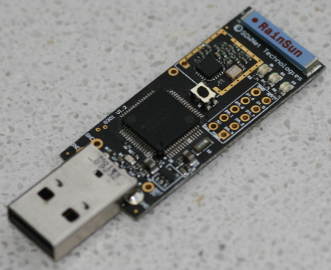
\includegraphics[width=0.5\textwidth]{img/gnode.jpg}
  \caption{The SOWNet's G-Node.}
  \label{fig:gnode}
\end{figure}
We took the position that further research would be enhanced if communication was possible between the watches and the G-Nodes\footnote{This way our testbed would become one of the largest academic deployment of wireless sensor nodes in the world, consisting of over 220 devices.}. Even though the CC1101 radio core used in G-Nodes is a stand alone product, recently it was also built into the members of the CC430 family of MCUs, hence the two are hardware-compatible. Adding this to the fact that we were time constrained, we decided to adapt the G-Node's radio stack implementation, so that it could run on Chronos. Having the same code on both types of devices provides maximum compatibility. We also made sure that this step was legitimate by complying with the license restrictions.

We do not present the detailed structure of the radio stack here because of its complexity. Instead we focus on our porting efforts. For details on the design of the ActiveMessage communication model please refer to \cite{BHC}, \cite{TEP116} and \cite{TEP126}.

The fundamental difference between the external CC1101 core and the built-in one lies in the way they communicate with the MCU. The standalone chip uses the SPI bus and some additional signal lines, while the internal core accepts commands through a register based interface. As we expected, almost everything else remains the same. It seems that TI has embedded the radio core into an MCU design and changed only the command interface.

Our modifications thus followed the same pattern. We removed all SPI related code from the HAL layer. Then, we changed the HAL code, to send all commands through appropriate registers. At that point, we were only missing the interrupts and status signals that were previously generated from signal lines coming from the radio chip. Interrupts were, however, easy to replace with native ones, sourced directly from the built-in core, while status signals could be read from registers via query commands (or in some cases, even directly). In the end, we cleaned up the code by removing some redundant definitions and adding comments documenting each command. Our final impression is that the built-in core is easier to manage than the external one.

The bulk of those changes were applied to the \emph{HalChipconControlP} module, which drives the radio core. It provides the \emph{HalChipconControl} interface, which can be used for low level radio operation. It gives the user precise control over transmission and reception, which might be necessary in some more sophisticated communication protocols.

During the development we encountered some serious difficulties. The biggest delay was caused by an elusive bug we introduced in the code. Namely, we called an interface function, rather than a local one that wrapped it. They had similar names, which made the difference difficult to notice. The function's purpose was to read the radio core's inner registers. However, without the use of the wrapper, a few of them were read incorrectly. This caused the radio to fail under some conditions, while working normally most of the time. We spent literally weeks, trying to find the source of the instability. At that point, we only had the LCD display to view the state of the watch and it only supported displaying numbers. Seeing that this was getting us nowhere, we started working on enabling the TinyOS \emph{printf} library. It helped a lot, allowing us to ascertain the exact condition at which the radio failed. After some investigation, we found that it happened during, seemingly harmless radio core register read. Finally, we noticed the misuse. That error was simple, but also very difficult to track down.

Another issue we had concerned G-Node interoperability. After porting G-Node's radio stack to Chronos, we expected that both would be able to communicate with each other. This wasn't the case though. We made sure that the transmission speeds matched, checked that G-Nodes were able to communicate among themselves and that Chronoses could do the same, but still they couldn't be mixed together. Finally, we found that the problem was rooted in the \emph{support/make/chronos.target} file. Namely, it didn't contain any definition of the \emph{DEFAULT\_LOCAL\_GROUP} constant. This caused the build system to impose a default value, different from the G-Node's default. In effect G-Node and Chronos used different values for the \emph{DEFAULT\_LOCAL\_GROUP}, and nodes from different local groups ignore each other's messages. We fixed it by defining the \emph{DEFAULT\_LOCAL\_GROUP} as empty, in the mentioned file. Interestingly, an empty environment variable is treated differently than an undefined variable. Some may view this as obvious, yet it caused us problems all the same.

Afters solving all problems, we've investigated the maximum length of the data that can be sent in one packet. In TinyOS this value is configured with the \emph{TOSH\_DATA\_LENGTH} constant. The size of the radio internal transmission/reception queue is 64 bytes. 11 are used for TinyOS packet header and 3 for the footer. This leaves 50 bytes for the payload. Interestingly, the radio seems to work even with this value set to 52. However we strongly recommend never to exceed 50.

\begin{figure}[h]
  \centering
  \includegraphics[width=1.0\textwidth]{diagrams/am_sender_c.eps}
  \caption{Overview of the \emph{AMSenderC} abstraction.}
  \label{fig:am_sender_c}
\end{figure}

Finally, note that the radio stack can be used through the interfaces provided by the \emph{ActiveMessageC}\footnote{This is an example of the Placeholder design pattern.} configuration. This however becomes less convenient if multiple message types are to be be sent and received. In such cases it is better to use the \emph{AMSenderC} generic component, shown in Figure~\ref{fig:am_sender_c}, which can be parametrized with the message type. It sends and receives only messages that have a particular id. At most one instance of this component in the system can use a given id, removing the risk of collisions. Moreover it provides a one-element message queue, which helps in arbitration between users of different message types, allowing them to forget about each others existence. For an excellent tutorial on how to use the radio stack in an application, see \cite{MoteToMote}. Also note that using the \emph{Low Power Listening} technique, supported by the radio stack, dramatically reduces power consumption. More on that can be found in \cite{LowPowerApps}.


\subsection{Centralized port management}

We noticed a bad practice TinyOS developers. Too often, various configurations, directly connect enumerated ports to components, like for example \emph{IO.Port31 -> SPI.ChipEnable}. This hides dependencies, making code much more difficult to understand and reuse. Moreover, experiments and modifications require a detailed review of schematics and datasheets to track the connections. Pin numbers neither indicate the MCU-side special function, nor the function of the pin on the other end. Continuing the above example, we don't know which peripheral device Port31 enables and if this port can even support the peripheral on the MCU side. It is difficult to ensure that one got the connections right, especially when they need to run crossover, like UART's TX and RX.

This matter becomes even more problematic in the case of CC430 MCUs, because they can dynamically reassign pin special functions. Moreover, doing this incorrectly blocks the ability of further port-mapping changes until the device is restarted. Thus, one faulty piece of code can break completely correct code. A source of such an error is difficult to track.

These issues lead to two conclusions. Firstly, it would be better to give ports mnemonics, describing their real purpose and use these abstract names in configurations. Secondly, port mapping should be done in one place. As both solutions need to be kept in sync, we believe that the best option is to join them, forming a centralized port management abstraction. Our implementation of this abstraction in Chronos took shape of the \emph{PlatformPortmapC} component. It provides IO pin interfaces named with the MCU pin special functions and ones representing the remote sides of the connections. Figure~\ref{fig:platform_portmap_c} shows the simplified structure of this component. Here it only provides access to two ports. \emph{CMA3000CSB} represents the accelerometer's chip-enable and \emph{CMA300MOSI} is its master-out slave-in SPI line. The \emph{UCB0SIMO} is a name of the special function assigned to the pin. It means that it acts as the slave-in master-out line, when USCI\_B0 submodule is configured to be an SPI interface. This function is assigned to Port16 by the \emph{PlatformPortmapP} module. PortJ is somewhat special. We had to add support for it to the  \emph{HplMsp430GeneralIOC} and its pins cannot have special functions assigned.

\begin{figure}[h]
  \centering
  \includegraphics{diagrams/platform_portmap_c.eps}
  \caption{The centralized port management in Chronos. (simplified)}
  \label{fig:platform_portmap_c}
\end{figure}

Now the accelerometer driver can use the \emph{CMA3000CSB} outlet to control chip-enable, while the USCI\_B0 driver connects to the \emph{UCB0SIMO}. All information about the actual circuit board connections is hidden in \emph{PlatformPortmapC}. This even gives potential for code portability. Another MCU from the CC430 family would only need an updated \emph{PlatformPortmapC} file to support the accelerometer\footnote{However, rarely is it that simple.}. Writing code for \emph{PlatformPortmapP} is also simplified because it only needs to realize mappings described in its parent configuration.

The solution described above is important for Chronos. All external connections, such as those in Figure~\ref{fig:chronos_schema}, use different hardware subsystems. This would not be possible without port management, because CMA3000-D01 and the USB debug dongle would have to share USCI\_A0.

\subsection{The serial connection support}

% through mspdebug bi-wire ?
% through radio packets ?

The serial port connection is the most reliable way for the MCU to communicate with the PC. It allows to relay packets between the tools on the PC and the radio mesh network. It also allows to receive network activity logs, to view its operation. And during the code development cycle, it allows to print messages from the MCU to a PC console, greatly reducing the debugging effort.

For Chronos, the best way to connect to a PC is to use the UART protocol in conjunction with the USB debug dongle. This protocol uses only two wires and is natively supported by the MCU hardware. There is however a small modification that needs to be done to the watch, to make it operational. The procedure is described, in detail, in Appendix \ref{appendix:uart_pins}.

Now we'll analyze how the serial stack is organized in TinyOS. Let's have a look at the main component of the \emph{tos/lib/serial} library. The \emph{SerialActiveMessageC}, depicted in Figure~\ref{fig:serial_active_message_c}, provides interfaces very similar to those of the radio stack.
\begin{figure}[h]
  \centering
  \includegraphics[width=0.6\textwidth]{diagrams/serial_active_message_c.eps}
  \caption{The \emph{SerialActiveMessageC} component. (simplified)}
  \label{fig:serial_active_message_c}
\end{figure}
We will not delve into them and refer the reader to \cite{TEP113} for details. This configuration relies on the \emph{SerialDispatcherC}, depicted in Figure~\ref{fig:serial_dispatcher_c}, to provide the \emph{SubSend} and the \emph{SubReceive} functionality.
\begin{figure}[h]
  \centering
  \includegraphics[width=0.75\textwidth]{diagrams/serial_dispatcher_c.eps}
  \caption{The \emph{SerialDispatcherC} component. (simplified)}
  \label{fig:serial_dispatcher_c}
\end{figure}
In \emph{SerialDispatcherC} there are three components engaged in the packet formation and transmission over a byte stream medium, but at the bottom lies the one most important to us - the \emph{PlatformSerialC}. It provides the \emph{UartStream} for byte transmission and the \emph{StdControl} for turning the connection on and off. Having this component is the key for a platform to support the serial communication. As the ports were already configured to the state shown in Figure~\ref{fig:chronos_schema}, by the \emph{PlatformPortmapC}, we only needed to get the USCI\_A0 module to act as an UART driver and provide an interface to it.

After some investigation, we've found the \emph{tos/chips/msp430/x2xxx/usci} library that supports USCI modules of some MSP430 MCUs. Most importantly, it configures the USCI and provides the \emph{UartStream} interface that we need. It isn't, however, directly compatible with the Chronos. There are some differences in register naming and interrupt sources, but not too big and we've managed to adapt it for our purposes. We didn't found a way to modify the library it self, without breaking other platforms, because the modifications were needed deep inside it and there was no way make the incompatible modules injectable. Instead we've copied it locally to the platform and changed what we needed. A crude solution but effective.

\begin{figure}[h]
  \centering
  \includegraphics[width=0.52\textwidth]{diagrams/platform_serial_c.eps}
  \caption{The \emph{PlatformSerialC} component.}
  \label{fig:platform_serial_c}
\end{figure}

The Figure~\ref{fig:platform_serial_c} presents the \emph{PlatformSerialC} component, that was the result of our work. The \emph{Msp430Uart0C} is the root component of the USCI library. It uses the \emph{Msp430UartConfigure} interface to retrieve the UART configuration parameters and in turn, it provides the \emph{Resource} interface, which is a part of the integrated concurrency and power management control mechanism and is used to gain access to the serial line. The \emph{ChronosSerialP} only stores the mentioned configuration parameters. All rest is done behind the scenes and as a result the \emph{SerialActiveMessageC} component is available. The \emph{tos/lib/printf} library uses it directly and therefore, we've also gained the ability to print messages on PC console. Details on how to use this library are described in Appendix \ref{ch:prog_env}.

Finally, note that, just as was the case with the radio stack, the recommended way of using the SerialActiveMessage communication is to instantiate a \emph{SerialAMSenderC} component for each message type.


\subsection{The accelerometer}

The CMA3000-D01 is an accelerometer chip, installed in Chronos. It allows to measure the acceleration, that the watch is subject to, at any given moment. This includes the Earth's gravity, which allows to estimate device's orientation in space. Also many modern smart-phone games are controlled, using accelerometer readings and some human activities can be recognized, solely based on its data. The CMA3000-D01 chip has three modes of operation. In the measurement mode, it sends a continuous stream of samples at a preconfigured rate. In the motion detection mode, the chip uses very little energy, while readily detecting any motions exceeding preconfigured thresholds. Similarly, in the free fall detection mode, it notifies the MCU whenever the acceleration readings falls below given thresholds. Overall, such sensor allows to create some very interesting applications.

However, this particular chips wasn't supported in TinyOS yet. This created an opportunity for us, to finally design some device drivers from scratch. During our work, we closely abided the recommendations of the Hardware Abstraction Architecture, therefore this code is our best example of its use. Also we've made the driver platform independent in the same way that the \emph{SerialActiveMessageC} is. The platform only needs to provide a proxy component bridging its SPI and GIO with the driver code.  This connection is realized by the \emph{PlatformCMA3kD0C} configuration, shown in Figure~\ref{fig:platform_cma3kd0_c}.

\begin{figure}[h]
  \centering
  \includegraphics[width=1.0\textwidth]{diagrams/platform_cma3kd0_c.eps}
  \caption{The bridge between the platform and the accelerometer driver.}
  \label{fig:platform_cma3kd0_c}
\end{figure}
Most importantly, it must provide the \emph{SpiPacket} interface that will allow to communicate with the CMA3000-D01 chip, along with the \emph{Resource} interface used to secure exclusive access to the bus. In addition it should also provide interfaces that give control over the IO lines that connect the MCU and the chip. These include the chip-select line, chip-power line and the chip-to-MCU interrupt line. While it is possible to use the accelerometer without control over their signals, doing so would reduce its functionality. In Chronos, this component instantiates the \emph{Msp430SpiB0C} to obtain the \emph{SpiPacket} interface. It originates from the same library that is used to support the serial connection. As shown in Figure~\ref{fig:chronos_schema}, the \emph{PlatformPortmapC} connects the USCI\_B0 subsystem to the accelerometer, therefore \emph{Msp430SpiB0C} indeed realizes the desired connection. The IO pin interfaces are sourced from the \emph{PlatformPortmapC} directly\footnote{Well almost, because the \emph{Msp430GpioC} adapter is used to convert the \emph{HplMsp430GeneralIO} interface to a platform independent \emph{GeneralIO}.}.

The interfaces provided by the proxy component are used in the Hardware Presentation Layer of our driver. Its members can freely instantiate and internally depend on the \emph{PlatformCMA3kD0C} component, because from the outside it is completely platform independent.
\begin{figure}[h]
  \centering
  \includegraphics[width=1.0\textwidth]{diagrams/hpl_cma3kd0_c.eps}
  \caption{The HPL of the accelerometer driver.}
  \label{fig:hpl_cma3kd0_c}
\end{figure}
Figure~\ref{fig:hpl_cma3kd0_c} shows all the components comprising the HPL. The most important abstraction, that is here created, is the accelerometer register access. It originates from the way that the accelerometer is controlled. There is only one frame, that can sent to it through the SPI. This frame contains a register address, a read-write bit and a data byte. If the bit indicates a write, than the accelerometer sets the specified register to the specified value and sends an answer frame, though it's not relevant in this case. It becomes relevant, however, if the bit was set to read, in which case, the answer caries the register value.

The main responsibility of the HPL is to abstract this mechanism, to allow for simple register modifications. We achieve this by splitting each register into the smallest meaningful portions, that we call subregisters, like the interrupt-enable bit or the 3 bits that configure the currently set accelerometer mode. HPL provides a simple interface that allows to set the value of a specific subregister, without changing the value of the whole register. Technically this violates the HPL contract because we must store some state in the components, but that's only necessary due to the split-phase nature of SPI communication. Had it been synchronous, than stack variables would suffice. More important than the lack of state is the primary purpose of the HPL, which is to provide clean interface to the hardware and we've definitely succeeded in that.  The second thing, that the HPL does, is the one time configuration of the interrupt line, because it's better to make it an input. Further responsibility for interrupt processing is left for the HAL, however.

Another HAL responsibility is the concurrency. Typically there will be more than one entity wanting to use the accelerometer. Also, one entity may with to use two of its functions consecutively. It could, for example, first wait for a motion and after it is detected, activate the more costly measurement mode. The drivers HPL doesn't have any notion of concurrency, though. Trying to make a second register access before the first one finises, will yield unpredictable results. Therefore, we've introduced the \emph{HalCMA3kD0OwnershipC} component, depicted in Figure~\ref{fig:hal_cma3kd0_ownership_c}.
\begin{figure}[h]
  \centering
  \includegraphics[width=0.85\textwidth]{diagrams/hal_cma3kd0_ownership_c.eps}
  \caption{The integrated concurrency and power management for the accelerometer.}
  \label{fig:hal_cma3kd0_ownership_c}
\end{figure}
It uses the mechanism demonstrated in Section \ref{ch:concurrency_and_power} to arbitrate the access to the HPL and the CMA3000-D01 chip it self. This is done via the \emph{Resource} interfaces it provides. Each user of the HPL must first request and be granted access to it. When the device isn't used, it is left under the control of the default owner, which is the \emph{HalCMA3kD0PowerManagerP} component. It is responsible for powering down the device, but it does so in an optimized manner. Instead of immediately cutting the power, it delays, waiting for a next user. This prevents an inefficient flickering behaviour when the accelerometer would have been turn on and off with high frequency. Now this frequency is bound by the inverse of the delay period. Note, however, that the default owner also requests and holds access to the SPI bus, so the delay shouldn't be too long.

This concurrency control and HPL form the foundation for higher level accelerometer abstraction implemented in the Hardware Abstraction Layer. It strives to expose most of the device capabilities to ensure maximal efficiency and performance. The design is organized around the three accelerometer operation modes. Each is supported by a separate HAL component that provides an interface specific to it. However, the broad configuration possibilities can be a flaw in more casual use or when platform independence is more important. Therefore, the Hardware Independence Layer provides components that wrap the HAL, configure the accelerometer to safe default values and provide easy to use and portable interfaces. The code supporting each accelerometer modes is very similar. Therefore we will only focus on how the measurement mode is implemented, because it will sufficiently cover the most important concepts.

Samples are always read by accessing three registers, containing components of the acceleration vector. In the measurement mode, however, the accelerometer not only tries to produce readings at a constant rate, but also notifies the MCU about readiness of a new sample, by changing the signal on the interrupt line. The MCU configures its GIO to monitor this line and fire an interrupt when the change is detected. This allows to read the sample as soon as it's ready, without wasteful pooling. Figure~\ref{fig:hil_accel_stream_c} shows the components supporting the measurement mode.
\begin{figure}[h]
  \centering
  \includegraphics[width=0.8\textwidth]{diagrams/hil_accel_stream_c.eps}
  \caption{The support for continuous acceleration measurements.}
  \label{fig:hil_accel_stream_c}
\end{figure}

The bulk of the logic is implemented in the \emph{HalCMA3kD0ContinousReadsP} module. It takes care of accelerometer configuration, handling the interrupts and reading the samples. The \emph{HalCMA3kD0ContinousReadsC} makes the necessary connections and hides unnecessary details. On top of it, the component of the HIL is built. The \emph{HalCMA3kD0ContinousReads} interface allows to configure both the rate at which samples will be taken and the precision scale.The \emph{HilAccelStreamP} hides these details, by setting the frequency to 40Hz and scale to maximum of 8g. It also requests the resource behind the scenes, so that the user can receive samples purely by the means of the simple \emph{Notify} interface.

\subsection{Persistent storage}

All applications, except the most basic ones, need non-volatile memory to perform their functions. Understanding this, we've decided that Chronos platform must provide some form of persistent storage. We tried to add support for it, however this proved more difficult than anticipated and we haven't succeed yet. This section describes how persistence is supported in the TinyOS and Chronos. We also draw lessons from our flawed design and ley plans for future work.

There is a well defined set of HIL interfaces meant to support non-volatile memory in TinyOS. Authors of \cite{TEP103} selected the three most common use cases and for each designed a custom abstraction. The first is represented by the \emph{ConfigStorageC} component and is used to store application's configuration, which usually is a set of small numeric values. The second, allows for the storage of large binary objects, through the \emph{BlockStorageC} configuration, which provides interfaces for efficient block reads and writes. The third is used to store logs. The \emph{LogStorageC} component ensures consistency of the records and supports circular logging.

However, the implementation of these interfaces was left fully in the discretion of the programmer, due to large variety of used flash chips and performance considerations. Authors recommend that each chip should have its own customized driver implementation and they do have a point, because Chronos has no flash chip at all. Nevertheless, we've decided that persistent storage is very important and must be supported somehow. Fortunately, it is possible to write to the MCU's internal flash memory in run time and therefore we can use a part of the program memory for application storage needs.

The flash memory of the watch is organized into three categories. The main program memory has 32KB and is divided into 512 bytes long segments. There is also the so called info memory, that has 4 segments, each 128 bytes long, and is meant specifically for configuration data. The last type of memory is used by the bootstrap loader and consists of 4 segments, each 512 bytes long. Now memory segmentation is very important, because segment is the minimal unit that can be erased. An erase sets all bits in a segment to 1. Writes can clear these bits to 0, but can never set a 0 to 1. This is the most important design consideration when dealing with flash memory.

An additional difficulty in Chronos, is the fact that any write to the flash memory, completely halts the MCU. This means that writes should be done in short bursts, to avoid delaying any pending tasks. Finally note, that as far as we know, the mass erase done during reprogramming, clears the main memory, but leaves the info and bootstrap loader segments intact. A subtlety that we've completely disregarded in our first approach to the driver implementation.

We've started by working out the low level details of the memory writing and erasing. The resulting component structure is shown in Figure~\ref{fig:hal_cc430_internal_flash_c}.
\begin{figure}[h]
  \centering
  \includegraphics[width=0.8\textwidth]{diagrams/hal_cc430_internal_flash_c.eps}
  \caption{The flash segment abstraction.}
  \label{fig:hal_cc430_internal_flash_c}
\end{figure}
It is organized around the concept of segments, being independent portions of the memory. This idea isn't bad, because it's convenient to assume that the whole segment can always be erased. The problem, however, is that it makes no distinction between them. Segments vary in size and the mass erase prevalence, but higher layers can not rely on these properties. Another issue is that, the \emph{writeBuffer} operation was made synchronous, which introduces lengthy tasks. Finally, the HPL has too much logic in it, making it effectively a HAL component. The code accesses registers directly, creating the exact clutter that HPL and HAL separation was supposed to avid. Overall, the internal flash HAL creates a leaky abstraction that tries to hide too many details, making subsequent use more difficult.

The HIL layer, in turn, is presented in Figure~\ref{fig:log_storage_c}.
\begin{figure}[h]
  \centering
  \includegraphics[width=0.8\textwidth]{diagrams/log_storage_c.eps}
  \caption{The HIL components of the driver.}
  \label{fig:log_storage_c}
\end{figure}
It consists of two very bulky components. The \emph{HilCC430LogReadWriteP} and the \emph{HalCC430CircularStorageC}, which are very tightly coupled together.
Multiple times we had to adjust the interface connecting them to implement their logic. The lacking lower layer, overly complicates the circular storage component. Moreover, note that there is no trace of any concurrency management, which is required by the specification. At that time, we understood very little of how TinyOS handles these issues. In practice the implementation worked poorly and eventually we've decided to abandon it.

To avoid all the above mistakes, we plan to employ test driven development during our second approach. Very recently this was made possible by \cite{TOSMock} and <tutaj nowy artykol Konrada>. This technique tends to produce smaller, more loosely coupled components with better interfaces and helps to find programming errors early in the development cycle. These are the virtues that the current implementation lacks.

% To enable wrapped line navigation:
% map j gj
% map k gk

% Vim settings:
% vim: set nonumber:
% vim: set spell:
% vim: set linebreak:
% vim: set wrap:
% vim: set textwidth=0:
% vim: set fo+=t:


\chapter{Evaluation}
\label{ch:evaluation}

As a part of our work we prepared and performed a series of experiments with eZ430.
This chapter describes the motivation, methodology and results of those tests.  

\section{Power usage}

\subsection{Official specification}
Texas Instruments provides a specification of the eZ430 battery life (see Table \ref{tab:power-specification}).
It contains detailed data about the power usage of sensors and the pre-built eZ430 applications: BlueRobin and SimpliciTI.
Both of the applications are controlled from a PC using the Chronos Control Center (Figure \ref{fig:chronos_control_center}).

\begin{table}[h]
  \centering
    \begin{tabular}{|l|r|r|}
        \hline
        \textbf{Mode} & \textbf{Average Current} & \textbf{Battery Life} \\ \hline
        Shelf mode (LPM4) & 2.7 $\mu A$ & 92.6 months \\ \hline
        Welcome screen on the LCD (LPM3) & 8.9 $\mu A$ & 28.0 months \\ \hline
        Time/Date on the LCD & 9.0 $\mu A$ & 27.7 months \\ \hline
        Continuous temperature measurement & 10.0 $\mu A$ & 25.0 months \\ \hline
        Continuous altitude measurement & 18.0 $\mu A$ & 13.8 months \\ \hline
        Continuous acceleration measurement & 166.0 $\mu A$ & 1.5 months \\ \hline
        Continuous BlueRobin RX & 40.0 $\mu A$ & 6.2 months \\ \hline
        Continuous SimpliciTI PPT (no button pressed) & 10.0 $\mu A$ & 25.0 months \\ \hline
        Continuous SimpliciTI SYNC & 0.9 $m A$ & 8 days \\ \hline
        Continuous SimpliciTI ACC & 3.7 $m A$ & 2 days \\ \hline
        1h/day BlueRobin RX & 10.3 $\mu A$ & 24.2 months \\ \hline
        1h/day SimpliciTI PPT (no button pressed) & 9.1 $\mu A$ & 25.4 months \\ \hline
        1h/day SimpliciTI SYNC & 46.1 $\mu A$ & 5.4 months \\ \hline
        1h/day SimpliciTI ACC & 169.9 $\mu A$ & 1.4 months \\ \hline
    \end{tabular}
  \caption{eZ430 Chronos estimated battery life (from Texas Instrument User's Guide \cite{eZ430Chronos})}
  \label{tab:power-specification}
\end{table}

\begin{figure}[h]
  \centering
  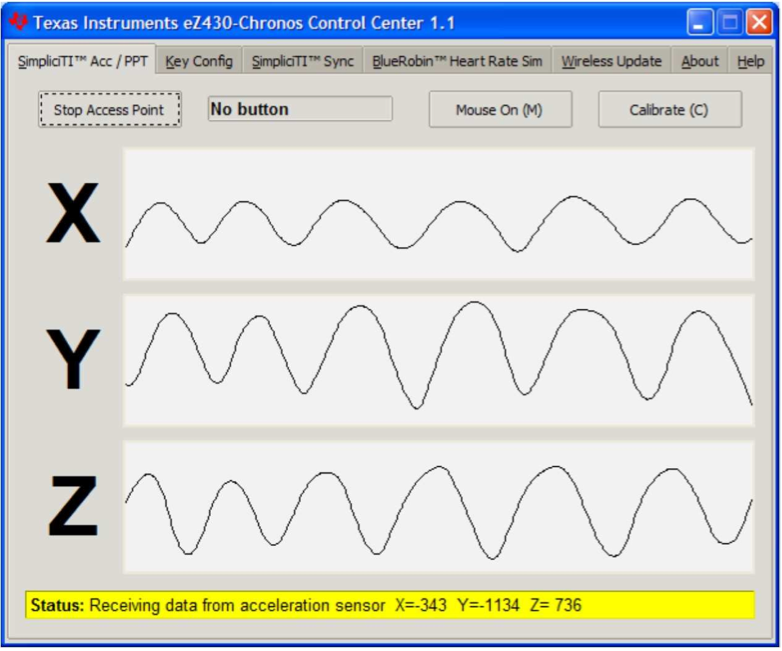
\includegraphics[width=0.6\textwidth]{img/chronos_app_control_center.png}
  \caption{Chronos Control Center PC Software (Courtesy of Texas
  Instruments)}
  \label{fig:chronos_control_center}
\end{figure}


BlueRobin\footnote{BlueRobin is a trademark of BM innovations GmbH} collects data from other ultra-low power sensors.
It supports retrieving heart beats from wireless belt.
In addition to that, it uses on-board eZ430 accelerometer to estimate speed and distance of person whose wear it.
Periodically, it transfers all those metrics through radio to a PC.
The application seems to be a proof of concept of watch for runners, similar to Adidas miCoach. 
It uses very little power, just a quarter of those required by using continously accelerometer alone.
However, it is impractical, because it requires user to be within radio range of a PC.

SimpliciTI\footnote{SimpliciTi is a trademark of Texas Instrument} is a versatile tool.
It consists of several modes.
PowerPoint Control mode (PPT) allows to map eZ430 buttons to PC keys.
That way a user can control a presentation, a music player, etc.
Acceleration data mode (ACC) enables transmitting eZ430 acceleration data to a PC through the radio.
It is also possible to control a PC mouse using the accelerometer data.
Synchronization mode (SYNC) allows for calibration of the device sensors and setting the time on eZ430 from a PC.
In addition to that, SimpliciTI provides standard watch functionality, such as clock, timer, alarm, etc. 

However, Important details, such as duty cycle and radio transfer rate are not specified for both applications.
Moreover, there are no data about the most power intensive operations: receiving and sending radio packets.
Such operations consume orders of magnitude more energy, than those listed in Table \ref{tab:power-specification}.
Therefore, having detailed measurements is required to do accurate battery life estimations.

\subsection{Low-power listening}
Overall, listening is usually the most power-expensive operation, largerly, because the majority of applications spend much more time listening than sending the data.
In order to reduce the listening time, TinyOS supports low-power listening (LPL).
However, sending data to node using LPL uses more energy.

In LPL, a listener node, periodically (e.g. every 200 ms) performs clear channel assasment (CCA).
If the check detects communication, it veryfies whether it is a sender's preamble.
If it is so, it starts regular radio listening, until the end of communication.

On the other hand, sender has to prelude its packet with a preamble of length at least equal to interval between listener's CCA checks.
A preamble is pre-defined by protocol and consist of repeated signal pattern.
That way, the listener node will always perform periodical check during sender's preamble and could easily identify it.
Having that, after the preamble, both nodes have turned on radio and the sender could transmit packet to the listener.

The example communication is showed in Figure \ref{fig:low_power_listening}.
In addition to that, nodes could continue communication, after the first sender's packet.
However, if there are no transmissions, both nodes return to the original state.
This allows to minimize overhead caused by preamble.

\begin{figure}[h]
  \centering
  \includegraphics[width=0.6\textwidth]{diagrams/low_power_listening.eps}
  \caption{Timeline of communication with low-power listening}
  \label{fig:low_power_listening}
\end{figure}

\subsection{Test setup and methodology}

\begin{figure}[h]
  \centering
  \includegraphics[width=0.4\textwidth]{diagrams/power.eps}
  \caption{Power measurement setup}
  \label{fig:power}
\end{figure}

% schema
Even though, we did not have a device that could measure electric current directly over time, we were able to calculate the current indirectly using Ohm's Law: 

$$
U = I \cdot R
$$

The law states that the potential difference on a resistor (U) is equal to the current (I) flowing through the resistor divided by its resistance (R).
In our setup, we knew the resistance of the resistor in Ohm and could measure the voltage drop using an oscilloscope (Figure \ref{fig:power}).
Therefore, we are able to calculate the electric current.
However, Ohm's law describes an ideal resistor.
In contrast, our testing setup does not fulfil all of the assumptions.
In particular, we a got a 20 $mV$ baseline difference in potential, which is subtracted from the final measurements.

The oscilloscope used was Owon PDS 5022S (see Figure \ref{fig:owon}).
It is capable of plotting voltage difference with a $ 0.1 ms$ accuracy.

\begin{figure}[h]
  \centering
  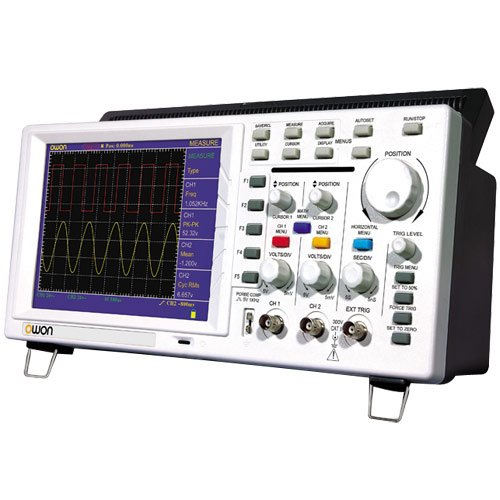
\includegraphics[width=0.4\textwidth]{img/owon_pds5022s.jpg}
  \caption{Owon PDS5022S oscilloscope (courtesy to the manufacturer)}
  \label{fig:owon}
\end{figure}

Instead of batteries, a 3 V direct current (DC) power adapter was used as the power source in order to provide a consistent voltage.

Having that setup we ran series of tests.
Each one begins with programming an eZ430 with a special purpose application, described in Table \ref{tab:power-apps}.
Every application ran for a few minutes, pausing the plot several times and recording the voltage difference.
A video was recorded for verification purposes.
As a final measure, we take the average of observations with a 1 $ mV $ accuracy.

For most of the tests the, the voltage drop was almost constant.
However, their are certain operations which could not be performed on eZ430 continuously.
In particular, sending series of radio packets is not possible without switching the radio to receiving mode between each transmission.
Therefore, the sending power consumption was measured only when actual packets were sent.

A similar issue appeared in low-power listening, where we measured the top power consumption of a receive check.


\begin{table}
  \centering
    \begin{tabular}{|l|l|}
        \hline
    \textbf{Application} & \textbf{Description} \\ \hline
    Null app & sleeps all the time \\ \hline
    LCDDriverTest App & uses LCD display intensively \\ \hline
    Loop & perform non-stop computations at 8 MHz \\ \hline
    TestAccelerator & Reads in a loop the acceleration reading, \\
    & unintentionally it is also maxing out CPU \\ \hline
    Radio listening & listen on radio (no difference whether it gets packets) \\ \hline
    Low-power listening & wakes every X $ ms $ to check if someone transmits on radio \\ \hline
    Sending at maximal power & sends packets with strongest signal - at +12 $ dB $ \\ \hline
    Sending at minimal power & sends packets with weakest signal - at -30 $ dB $ \\ \hline
    \end{tabular}
  \caption{Special purpose application used to measure power usage}
  \label{tab:power-apps}
\end{table}

\subsection{Results}

Our equipment was good enough to measure radio-related operations with a reasonable accuracy (see Table \ref{tab:power-usage}).
In contrast, the onboard sensors consume too little energy to be above the noise.

However, our results are complementary to the official specification.
Combing both data sources it is possible to estimate the energy budget of a real-world application.

For example, we might assume that our application will listen for $2 \%$i of the time, send for $ 0.1 \% $ and use accelerometer for $ 10 \% $.
Under these assumption, the estimated average power usage of the application will be:
\begin{equation}
0.1 \% \cdot 27 mA + 1 \% \cdot 10 mA + 10 \% \cdot 166 \mu A + 90 \% \cdot 8 \mu A = 0.1508 mA   
  \label{eqn:power_example}
\end{equation}
Which gives a battery life of:
$$
\frac{190}{0.1508} \approx 1260 h \approx 52 days
$$
(assuming 190 mAh CR2032)



\begin{table}[h]
  \centering
    \begin{tabular}{|l|r|r|r|}
        \hline
              & \textbf{I (estimated)} & \textbf{I (measured)}          & \textbf{Voltage drop on resistor}  \\ \hline
Baseline & - & - & 20 $ mV $ \\ \hline
Null app    & - & 3 $ mA $          & 20 $ mV $  \\ \hline
LCDDriverTest app    & - & 3 $ mA $ & 20 $ mV $  \\ \hline
Loop    & 1 $ mA $ & 4 $ mA $          & 28 $ mV $  \\ \hline
TestAccelerator     & 1 $ mA $ & 4 $ mA $          & 28 $ mV $  \\ \hline
Radio listening     & 16 $ mA $ & 19 $ mA $   & 130 $ mV $  \\ \hline
Low-power listening     & 10 $ mA $ & 13 $ mA $              & 88 $ mV $  \\ \hline
Sending at maximal power     & 27 $ mA $ & 30 $ mA $              & 206 $ mV $  \\ \hline
Sending at minimal power      & 12 $ mA $ & 15 $ mA $            & 102 $ mV $  \\ \hline

    \end{tabular}
  \caption{eZ430 Chronos measured battery life}
  \label{tab:power-usage}
\end{table}

\subsection{Energy cost of low-power listening}

Listening and sending the data takes roughly the same amount of power as described in Table \ref{tab:power-usage}.
Also sending a preamble consumes the same amount of power as sending the data.
The only unknown is thus how much power a receive check costs.

A single check uses clear channel assessment, which could give a false positive, but uses less power than listening.
It takes 4 $ ms $ with the average 5 $ mA $ current during the whole check (see Figure \ref{fig:low_power_receive_check}).

\begin{figure}[h]
  \centering
  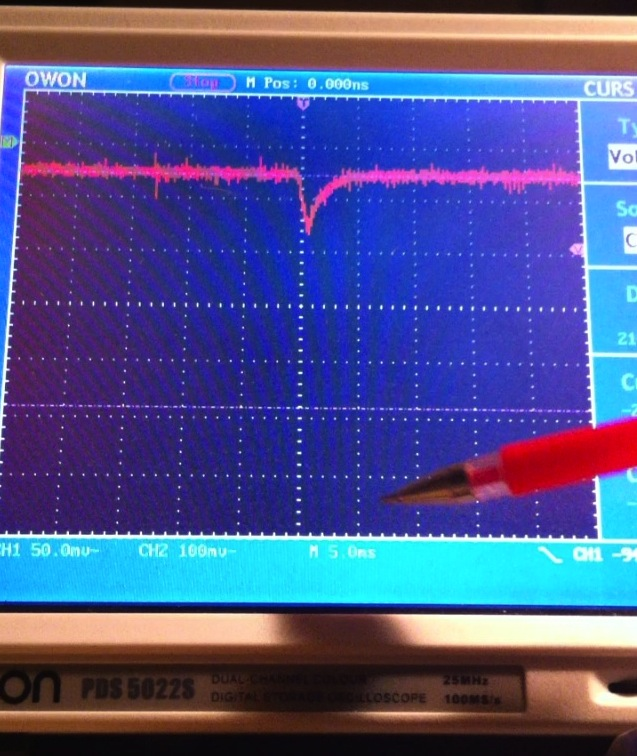
\includegraphics[width=0.6\textwidth]{img/low_power_receive_check.jpg}
  \caption{Inverted graph, low peak: $ 88 mV$, top line: 20 $ mV $}
  \label{fig:low_power_receive_check}
\end{figure}

For example, idly listening with LPL with a 250 $ ms $ sleep interval consumes:
$$
\frac{4 \cdot 4 ms \cdot 5 mA}{1000 ms} \approx 0.08 mA
$$
In addition to that, we need to calculate the power consumption of an actual transfer.
Let say we transfer take 50 $ ms $ every 30 $ s $, also we will be listening on average half of the preamble: $\frac{250 ms}{2} =  125 ms$.

So the listener uses:
$$
\frac{(125 ms + 50 ms) \cdot 16 mA}{30 \cdot 1000 ms}  + 0.08 mA \approx 0.09 mA + 0.08 mA = 0.17 mA
$$

While sender node uses:
$$
\frac{(250 + 50) ms \cdot 30 mA}{30 \cdot 1000 ms} \approx 0.3 mA
$$

\subsection{Other considerations}
In the real world, there are many other factor that affect the battery life.
For example, battery capacity depends on temperature and is usually lower than are specified by the manufacturer.
Because of that, real world applications have shorter battery lives than what estimations would suggest.


\section{Radio range}

Range is one of the most important parameters of a radio module.
However, there is no official specification of the eZ430 range.
The user documentation (\cite{eZ430Chronos}) gives only a vague description:
\begin{quote}
In free field distances of up to 100 m (328 ft) have been measured. The range in other conditions,
especially within buildings, is hard to predict.
\end{quote}

That kind of description is definitely not sufficient.
As an application developer, we are interested not only in the maximum range, but also in the transfer reliability.


\subsection{Methodology}

As part of the evaluation we did line-of-sight tests in a park.
We used two watches that could ``see'' each other, with no objects between them.
Radios were configured for the 868 MHz frequency with a 250 kbit transmission rate.
All watches were fully assembled and placed about 80 $ cm $ above the ground.
The power was supplied by previously unused CR2032 batteries, which were replaced in the middle of the tests to provide a more consistent environment.

The test consisted of sending 100 20-byte packets.
Between each packet, there was a 256 $ ms $ sleeping interval.
During the test s watch was rotated to simulate real hand movements.
After each test, the data was sent to a PC using radio printf and a GNode as a bridge.

It took a few iteration to produce results which were repeatable.
Tests inside of building, without line-of-sight, with used batteries or with fixed watch rotation result in inconsistent or hard to reproduce data.

All these tasks were performed using a ChronosConnectivityAssesment application.
The application provides a user interface using the LCD and buttons.
One of it its features is the ability to change the radio output power level.

For all tests we collected the following three metrics:
\begin{itemize}
  \item \textbf{reliability} --- packets received
  \item \textbf{average RSSI} --- the amount of received signal strength indication (RSSI), provided by hardware.
  \item \textbf{average LQI} --- Link quality indicator (LQI), a heuristic quality value provided by the radio chip.
\end{itemize}

Each test were performed with three different radio strength: +12 dB (maximal), 0 dB and -30 dB (minimal).

All distances are in meters, except the one denoted ``next''  which meant closest possible within a given radio strength.
Placing two watches closer than this distance disables radio communication completely.
``Next'' is about $20 cm$ for $+12 dB$ and close to $0 cm$ for $- 30 dB$.

% methodology

% Chronos connectivity

\subsection{Reliability results}

The results data show that radio got range of about $50$ meters.
Within short distance, there are very few packets lost\footnote{in our environment there are almost no collisions}.
However, There is a sharp drop in reliability after certain distance.
This is excepted, as free-space path loss is square proportional to the distance from the source.

Although, radio strength -30 dB may seems impractical, it is a good method to detect whether sender is close ($< 2m$) to the receiver.

Overall, radio chip in eZ430 is relaible and provide reasonable radio range.


\subsubsection{+12 dB}

\begin{figure}[H]
  \centering
  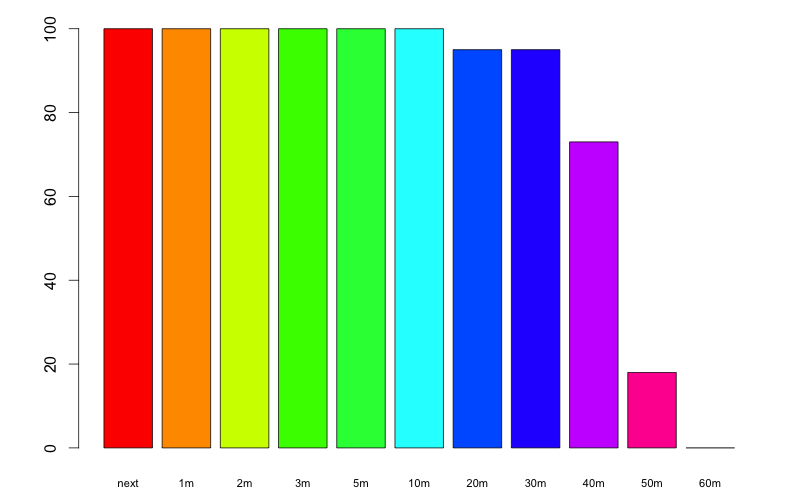
\includegraphics[width=0.9\textwidth]{img/tests/range/db_12.png}
\end{figure}


\subsubsection{0 dB}

\begin{figure}[H]
  \centering
  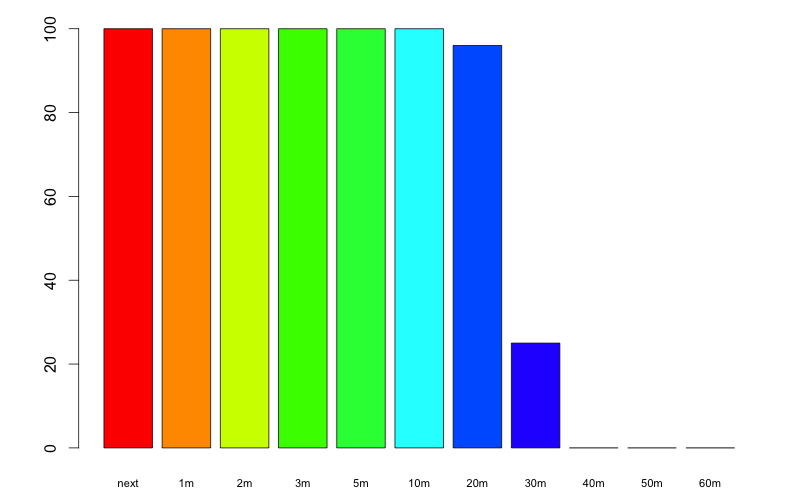
\includegraphics[width=0.9\textwidth]{img/tests/range/db_00.png}
\end{figure}

\subsubsection{-30 dB}

\begin{figure}[H]
  \centering
  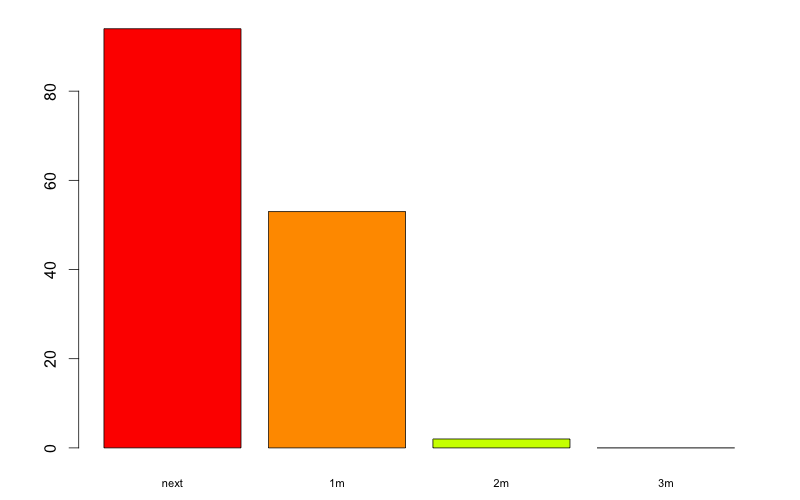
\includegraphics[width=0.9\textwidth]{img/tests/range/db_m30.png}
\end{figure}

\subsection{RSSI results}


The RSSI results are presented as box plots.
The thick line shows the median.
The box edges are on 1st and 3rd quartile.
The top and bottom lines are correspondingly the minimal and the maximal element.
Each point which is more than 1.5 times away than the height of the box is considered as an outlier and marked with a circle.

RSSI is usually used to determine the quality of radio communication.
It may be also utilized to estimate the distance between a sender and a listener.
Though, single measurement may be misleading, a median from series of transmissions is a good indicator.


\subsubsection{+12 dB}

\begin{figure}[H]
  \centering
  \includegraphics[width=0.9\textwidth]{img/tests/rssi/db_12.png}
\end{figure}


\subsubsection{0 dB}

\begin{figure}[H]
  \centering
  \includegraphics[width=0.9\textwidth]{img/tests/rssi/db_00.png}
\end{figure}

\subsubsection{-30 dB}

\begin{figure}[H]
  \centering
  \includegraphics[width=0.9\textwidth]{img/tests/rssi/db_m30.png}
\end{figure}

\subsection{LQI results}
The LQI results have same form as the RSSI results.

LQI is an alternative metric to RSSI.
Even from a signal LQI data point gives a good prediction of packet loss.
However, it is a bad metric to estimate the distance and RSSI should be used for that purpose instead.


\subsubsection{+12 dB}

\begin{figure}[H]
  \centering
  \includegraphics[width=0.9\textwidth]{img/tests/lqi/db_12.png}
\end{figure}


\subsubsection{0 dB}

\begin{figure}[H]
  \centering
  \includegraphics[width=0.9\textwidth]{img/tests/lqi/db_00.png}
\end{figure}

\subsubsection{-30 dB}

\begin{figure}[H]
  \centering
  \includegraphics[width=0.9\textwidth]{img/tests/lqi/db_m30.png}
\end{figure}

% results

\section{Radio throughput}

% methodology
The theoretical throughput is 250 kbits.
However, the communication requires sending frame headers and footers.
In addition to that, the radio driver performs clean channel assessment before each transfer.
This reduces packet collisions, but reduce the bandwidth.

% results
Using the maximal packets size (63 bytes) we sent 8000 packets as fast as possible.
It took 45 seconds, which gives 11.2 kB/s as the measured transfer.
Provided that two watches were close enough, such that there are no packets lost.


\section{Sample application: Zordon}

Also as part of evaluation, we implemented sample application.
Each watch is associated with a name and has the radio in low-power listening mode.
A user select one of the names from the LCD menu, then he could send a beep request over radio.
If the watch receives beep request addressed to its name, it plays a sound using a built-in buzzer and displays the sender's name.

This application can be used to call friends who are in nearby rooms.
It is a useful example which shows the major TinyOS advantage: it allows to write application just by describing its logic without worrying about underlying hardware.



% Use case


% \Bump

% \ CTP


% \chapter{Applications for Chronos}


\chapter{Conclusions and further work}

\section{Conclusions}

% Complete environment

The aim of this project was to provide infrastructure to evaluate routing algorithms in mobile sensor networks.
It was accomplished by porting TinyOS to eZ430 Chronos, which is the first mobile node supported by this operating system.

Our work start from scratch, without essential programming tools.
Reusing existing software, we assembled convenient development environment, which consist of compiler, debugger, chip programmer, printf library, build system, IDE and virtual machine.
The core part of our work was implementation of TinyOS device drivers for eZ430 in nesC programming language.
We also performed several evaluation in order to test radio power consumption, range and throughput.
At last, but not at least, we provided example application --- Zordon for Chronos, which demonstrate its hardware features..

Although the project may seem to be limited to low-level programming, it delivered a robust, well-designed abstraction, which encapsulate eZ430 technical details.
It is a radical improvement over manufacturer's tools, which require handling manually hardware issues and are suitable only for simple applications.
Our programming environment supports modular, object-oriented, cross-platform applications.
In addition to that, it is possible to take advantage of TineOS ecosystem:
ready to use applications as well as tools and libraries (e.g. unit-test framework \cite{TOSMOCK}).

We believe it is the great leap forward in development of applications for mobile sensor networks.

% complete programming environment

\section{Further work}
There are a lot of research projects which could take advantage of our TinyOS port to eZ430.
Especially two of them seems to be a next step.

\subsection{Evaluations of existing routing protocols}
There are many published articles about sensor network protocols which were implemented in TinyOS.
However, there was no mobile hardware nodes to evaluate them in non-static environment.
Using our TinyOS port to eZ430 it is much easier to perform that kind of experiments and provide valuable results for the research community.

\subsection{Better low-power listening}
Low-power consumption is one of the key requirements for sensor nodes.
Radio communication usually use most of the energy, so it is the best candidate for further optimizations.
The savings are achieved by turning off radio module whenever it is possible.
However, deciding when radio listening is needed is a hard problem.
The eZ430 Chronos has implementation of low-power listening, but it is based on simple algorithm.

Various scientific papers presents more sophisticated solutions \cite{BMAC} and \cite{DCCLPL}.
Their power performance is claim hardware and application specific.
Although, implementation and evaluation of those algorithms would require significant amount of work, it is likely that they would be substantial better implementation of low-power listening.


% we need a better MAC layer


\appendix

\chapter{Assembling programming environment}

% SPI wire programming

\subsection{Bug and limitations}

% connected to TOS build

\section{Mspdebug}

\section{Printf library}
\label{sec:printf_library}

When a code is first written, more often than not, it does not work as
expected. Unit testing helps, but often errors arise from making false
assumptions and these may be reflected in tests as well. In such case,
only observing the actual behaviour during execution will lead to
fixing the issue.

But how to observe the behaviour of a wireless sensor node after it
has been flashed with a new executable image?

One way is to observe LEDs on the circuit board.  In case of the
chronos watch, which has no LEDs, LCD display can be used instead, to
even better results. But only small amount of information can be
retrieved through through such a channel. Another possibility is to
use mspdebug tool mentioned before.  However if you ask a computer
programmer which tool he most commonly uses to find out what's
happening in his program, \emph{the debugger} will be his second
answer. The first would be \emph{printf}.

TinyOS has a convenient printf library that allows sending text
messages from running device to the PC and display them in a console.
Its use is simple and comprises of following steps:

\begin{itemize}
  \item Include the printf library files to the build, by adding
    following line to your Makefile:

    \texttt{CFLAGS += -I\$(TOSDIR)/lib/printf}

  \item Optionally, increase the printf buffer size (250 bytes by
    default), by adding following line to your Makefile:

    \texttt{CFLAGS += -DPRINTF\_BUFFER\_SIZE=<NEW\_SIZE>}

  \item Instantiate printf components in your application
    configuration. This step depends on which implementation of
    printf you use. See following sections for details.

  \item Add following include in the file you wish to use printf in:

    \texttt{\#include ``printf.h''}

  \item Use \texttt{printf} statement to display messages and
    occasionally \texttt{printfflush} to ensure that they are not stuck
    in a buffer.

    \texttt{printf(``Value is \%d\textbackslash n'', value);} \\
    \texttt{printfflush();}

  \item To receive the messages you will need to run the printf
    client. How this is done also depends on which implementation of
    print you use.
\end{itemize}

Now before we delve in to the specific implementations there's a warning
regarding printf buffering. Only after the buffer is filled or when
you call \texttt{printfflush} does the data get actually sent to the
PC. This isn't however immediate. If you very quickly print more text
than the capacity of the buffer, some of the messages will be lost!
Also note that \texttt{printfflush} is non-blocking and after calling
it, the buffer may still be full for a while, and thus messages
may still get lost.

To overcome this,  you can shorten your messages, slow down printing
rate to ensure enough time to transmit current contents of the buffer
or increase the size of the buffer.

\subsection{Mspdebug printf}

\subsection{Radio printf}

\subsection{Serial port printf}
Third version of the printf library uses the serial port connection to
communicate with the PC. On the watch end it uses the UART (Universal
Asynchronous Receiver/Transmitter) hardware driver. This has both
serious advantages and a disadvantage.

Main advantage is, that serial communication is most reliable and best
supported way of sending printf messages in TinyOS. For example the
PrintfClient tool that comes with vanilla TinyOS, handles receiving
the packets and displaying them in the console. Also it is the least
intrusive one, since it neither requires halting the MCU nor sending
packets through the radio transceiver.

Main drawback however is that Texas Instruments did not make the UART
pins easily accessible on the chronos circuit board and certain
hardware modification is necessary to reach them. How to perform it,
is described in Appendix \ref{appendix:uart_pins}. Fortunately, no
additional hardware besides the USB debug interface is necessary after
the modification is done.

To enable this version of printf library you need to augment
instructions given in section \ref{sec:printf_library} with following
steps:

\begin{itemize}
  \item Instantiate these components in your application configuration:

  \texttt{components PrintfC, SerialStartC;}

  \item Connect the watch with hardware modification described in
    Appendix \ref{appendix:uart_pins} to the USB debug dongle and
    connect the dongle to the PC.

  \item To receive messages run PrintfClient:

  \texttt{java net.tinyos.tools.PrintfClient -comm serial@/dev/ttyACM0:chronos}

  Note that watch may have shown in \texttt{\textbackslash dev} under
  different name, most commonly
  \texttt{\textbackslash dev\textbackslash ttyACM1}
\end{itemize}

\section{Eclipse integrated development environment}

The most practical way to work with TinyOS code is using the Eclipse
IDE. Some great work has been done on that field, resulting in the Yeti 2
plugin. It supports TinyOS application and platform development,
providing many features. Below we'll describe the most important ones.

Firstly, in editor, there is some very good {\bf code completion} available
which eases writing both module and configuration files. It completes
component instantiations and connections. Also it completes interface
calls, function calls and variable names, and after adding a
\texttt{uses} or \texttt{provides} declaration, it offers to create
command and event stubs. These features are best shown on the
following series of Figures, \ref{fig:first_compl} through
\ref{fig:last_compl}.

\begin{figure}[h]
  \centering
  \includegraphics[width=0.85\textwidth]{img/eclipse_compl1.png}
  \caption{Component instantiation completion.}
  \label{fig:first_compl}
\end{figure}

\begin{figure}[h]
  \centering
  \includegraphics[width=0.8\textwidth]{img/eclipse_compl2.png}
  \caption{User connection completion.}
\end{figure}

\begin{figure}[h]
  \centering
  \includegraphics[width=0.9\textwidth]{img/eclipse_compl3.png}
  \caption{Provider connection completion.}
\end{figure}

\begin{figure}[h]
  \centering
  \includegraphics[width=0.9\textwidth]{img/eclipse_compl4.png}
  \caption{Interface completion.}
\end{figure}

\begin{figure}[h]
  \centering
  \includegraphics[width=0.9\textwidth]{img/eclipse_compl5.png}
  \caption{Command completion.}
\end{figure}

\begin{figure}[h]
  \centering
  \includegraphics[width=0.9\textwidth]{img/eclipse_compl6.png}
  \caption{Command stubs generation.}
  \label{fig:last_compl}
\end{figure}

Another very useful feature, especially for a new developer wishing to
familiarize himself with TinyOS structure is the {\bf component
explorer}. It graphically displays components instantiated and
interconnected in configurations. Interfaces can be viewed as well.
Starting at the top level application configuration, every part of
it's code can be reached. This is by far the most efficient way to
explore the call hierarchy and find where particular functions are
implemented. Example of the PrintfC configuration, viewed through
the component explorer is shown in figure
\ref{fig:eclipse_compexp}.

\begin{figure}[h]
  \centering
  \includegraphics[width=0.7\textwidth]{img/eclipse_compexp.png}
  \caption{Component explorer showing PrintfC configuration.}
  \label{fig:eclipse_compexp}
\end{figure}

The eclipse editor also gives many warnings about the code without
triggering compilation. Moreover many of these useful warnings are not
raised by NesC compiler, which is an added value. 

Finally, one of the most useful parts of Yeti 2 is {\bf the debugger}.
The chain of tool invocations, needed to debug an application on the
chronos watch is long, but running them is as easy as pressing a
button in the IDE. At the lowest level, the \emph{mspdebug}
communicates with the watch through the USB debugging dongle. It runs
a GDB Server to which newer versions of \emph{msp430-gdb} are able to
connect. Eclipse runs this last executable and forms practical data
views, reading crude data from GDB. Here is a list of most useful
views and features:
\begin{itemize}
  \item Single stepping through code in NesC editor.
  \item Call stack view.
  \item Breakpoints list (though limited to 3 active at any moment).
  \item Disassembly view.
  \item Raw memory view.
  \item Registers view.
  \item Local variables view.
  \item Module variables view.
\end{itemize}

Yetti 2 provides many more functions not mentioned here, most of which
are standard to Eclipse IDE and expected to be available for any
supported programming language. Developer naturally explores them
while using the IDE.

The installation is described in Appendix \ref{appendix:env_install}
and a preconfigured setup is available in the virtual machine
distributed with this work.

\section{Console centric development}

It is also possible to develop TinyOS code without using any
IDE\footnote{In fact, this is exactly how TinyOS was first written.}.
To support such style of development two changes were necessary.
Firstly, the environment variables were configured to point to the
TinyOS source code locations and Makefile rules. This makes it
possible to use make command to build applications. Secondly, syntax
and indentation configurations files for vim were added to ensure
convenient and practical code editing.  Having both working make and
good text editor allows for development almost as efficient as with
the Eclipse IDE. The only setback is that if the developer is not
familiar with TinyOS naming, he will not receive aid from code
completion.

\section{Development virtual machine}

The setup of all the tools needed to work on the TinyOS Chronos
platform and application code, is complicated and takes time. To ease
this step for new developers, a virtual machine image was created.
All the tools have been installed in it and configured, to work
out-of-box. The most recent version of the source code is checked out
and imported into Eclipse IDE, with a run configuration ready to build
and install TinyOS Blink application.  All that is left to the user,
is connecting the watch through the USB debug interface and pressing
Run button.

% Vim settings:
% vim: set textwidth=70:
% vim: set fo+=t:


% TODO: write appendices
\appendix
\chapter{Hardware modification enabling serial communication}
\label{appendix:uart_pins}

Here we describe the steps necessary to enable serial communication
between the watch and the PC. On the PC side, serial port will be
emulated through USB, by the same USB debug dongle that is used to
flash program images on the watch. It is a very convenient solution.

We'll start by looking and the USB dongle. Figure
\ref{fig:chronos_dongle_pins} shows the function of the dongle pins.
\begin{figure}[h]
  \centering
  \includegraphics[width=0.7\textwidth]{img/chronos_dongle_pins.png}
  \caption{Pin functions of the USB debug dongle (Courtesy Texas Instruments)}
  \label{fig:chronos_dongle_pins}
\end{figure}
Ones labeled \emph{UART TX} and \emph{UART RX} are responsible for
serial communication. However if you look at chronos watch schematics,
you'll see that these pins remain unconnected in the watch. Relevant
snippet is shown in figure \ref{fig:chronos_unonnected_uart}
\footnote{Schematics are published in \cite{eZ430Chronos} and also
shown in appendix \ref{appendix:watch_schematics} for quick
reference.}.
\begin{figure}[h]
  \centering
  \includegraphics[width=0.15\textwidth]{img/chronos_unonnected_uart.png}
  \caption{Unconnected UART pins on the watch (Courtesy Texas Instruments)}
  \label{fig:chronos_unonnected_uart}
\end{figure}
This is exactly what needs to be changed. Fortunately the MCU is
capable of dynamic port remapping. This means that these UART pins may
be connected to any two IO pins and software can handle rest of the
configuration.

IO pins that are mostly easily connected to the serial lines are those
responsible for watch buttons. The exact location of the connections
is presented in figure \ref{fig:chronos_where_to_connect}.
%TODO(horban): Image goes here
Now we'll describe exact steps necessary to perform the modification:
\begin{itemize}
  \item Take off the  part of the cover that comprises battery compartment.
    Loosen the couplings with a small screwdriver as shown in figure
    \ref{fig:chronos_cover_off}. Ensure you do not lose two tiny
    golden springs that connect power and buzzer to the board.
    %TODO(horban): Image goes here
  \item Prepare two short pieces of wire that will make the
    connections. Take off the isolation. Make sure their length is
    comfortable. Shape them until they form smooth paths between the
    connection points. Ensure that they will not contact to any other
    elements of the watch (SMT resistors near the connector).
  \item Place one of them in position and secure it with tape
    from one side.
  \item Solder the other side to the board. Bonding will now hold the
    wire in position. Remove the tape and solder the other end.
  \item Solder the second wire the same way. End result should
    look similarly to figure \ref{fig:chronos_with_wires}.
    %TODO(horban): Image goes here
  \item Put the cover back on. Ensure that two small golden springs
    are in position.
  \item Test the device, by running TinyOS TestSerial application. See
    it's \emph{README.txt} file for detailed instructions.
\end{itemize}

Note that certain unreliability of the serial port is to be expected.
1 : 1500 error rate is well within tolerance.

%------------------------------------------------------------------------------

\appendix
\chapter{Chronos watch schematics}
\label{appendix:watch_schematics}

\begin{figure}[h]
  \centering
  \includegraphics[width=1.0\textwidth]{img/watch_schematics.png}
  \caption{(Courtesy Texas Instruments)}
\end{figure}

\appendix
\chapter{Chronos development environment installation}
\label{appendix:env_install}


% Vim settings:
% vim: set textwidth=70:
% vim: set fo+=t:


\begin{thebibliography}{99}
\addcontentsline{toc}{chapter}{Bibliography}

\bibitem[BerkDB]{berkdb}
  M. A. Olson, K. Bostic and M. Seltzer,
  \textit{Berkeley DB},
  In USENIX (June 1999), pages 183-192

\bibitem[Liu2009]{liu2009long}
  Liu, N.H. and Wu, C.A. and Hsieh, S.J.,
  \textit{Long-Term Animal Observation by Wireless Sensor Networks with Sound Recognition},
  Wireless Algorithms, Systems, and Applications (2009)

\bibitem[InternetOfThings]{InternetOfThings}
  Kevin Ashton,
  \textit{That 'Internet of Things' Thing},
  RFID Journal (July 2012) \url{http://www.rfidjournal.com/article/view/4986}

\bibitem[GuArtNet]{GuArtNet}
  GuArtNet whitepaper \url{http://www.sownet.nl/download/GuArtNet\_Whitepaper\_English.pdf}

\bibitem[Klues et al.]{Klues et al.}
  Kevin Klues, Vlado Handziski, Chenyang Lu, Adam Wolisz, David Culler, David Gay, and Philip Levis. 2007.
  \textit{Integrating concurrency control and energy management in device drivers.}
  In Proceedings of twenty-first ACM SIGOPS symposium on Operating systems principles (SOSP '07). 

\bibitem[singhvi2005intelligent]{singhvi2005intelligent}
  Singhvi, V. and Krause, A. and Guestrin, C. and Garrett Jr, J.H. and Matthews, H.S.,
  \textit{Intelligent light control using sensor networks},
  Proceedings of the 3rd international conference on Embedded networked sensor systems (2005), pages 218-229

\bibitem[NesC]{NesC}
  David Gay, Philip Levis, and Robert von Behren.
  \textit{The nesC Language: A Holistic Approach
  to Networked Embedded Systems}.  \newblock In
  {\em Proceedings of the ACM SIGPLAN 2003
  Conference on Programming Language Design and
  Implementation (PLDI)}, 2003.

\bibitem[NesCMan]{NesCMan}
  David Gay, Philip Levis, David Culler, Eric Brewer,
  \textit{nesC 1.1 Language Reference Manual},
  May 2003 \\
  \url{http://www.tinyos.net/tinyos-1.x/doc/nesc/ref.pdf}


\bibitem[TOSMock]{TOSMock}
  Piotr Glazar, \textit{A unit-testing framework
  for wireless sensor networks.} \\ Master thesis,
  University of Warsaw (2012)

\bibitem[MM]{MM}
  Mateusz Michałowski, \textit{An Experimental Platform
  for Wireless Sensor Networks} \\ Master thesis,
  University of Warsaw (2012)

\bibitem[TOSSIM]{TOSSIM}
  P.~Levis, N.~Lee, M.~Welsh, and D.~Culler.
  \textit{Tossim: accurate and scalable
  simulation of entire tinyos applications.}
  \newblock In {\em SenSys '03: Proceedings of the
  1st international conference on Embedded
  networked sensor systems}, pages 126--137, New
  York, NY, USA, 2003. ACM.

\bibitem[TinyOS]{TinyOS}
  Levis, P. and Madden, S. and Polastre, J. and Szewczyk, R. and Whitehouse, K. and Woo, A. and Gay, D. and Hill, J. and Welsh, M. and Brewer, E. and others,
  \textit{TinyOS: An operating system for sensor networks}
  Ambient intelligence (2005)

\bibitem[DCCLPL]{DCCLPL}
  Christophe J. Merlin, Wendi B. Heinzelman
  \textit{Duty Cycle Control for Low-Power-Listening MAC Protocol}, 2010 

\bibitem[BMAC]{BMAC}
  Joseph Polastre, Jason Hill, David Culler
  \textit{Versatile Low Power Media Access for Wireless Sensor Networks}
  SenSys '04 Proceedings of the 2nd international conference on Embedded networked sensor systems (2004)


\bibitem[TOSProg]{TOSProg}
  Philip Levis, \textit{TinyOS Programming}, October 27, 2006 \\
  \url{http://www.tinyos.net/tinyos-2.x/doc/pdf/tinyos-programming.pdf}

\bibitem[BHC]{BHC}
  Philip Buonadonna, Jason Hill, David Culler,
  \textit{Active Message Communication for Tiny Networked Sensors}, 2001 \\
  \url{https://koala.cs.pub.ro/redmine/attachments/156/ammote.pdf}

\bibitem[TEP2]{TEP2}
  Vlado Handziski, Joseph Polastre, Jan-Hinrich Hauer, Cory Sharp,
  Adam Wolisz, David Culler, David Gay, \textit{Hardware Abstraction Architecture}, September,  2004 \\
  \url{http://www.tinyos.net/tinyos-2.x/doc/pdf/tep2.pdf}

\bibitem[TEP103]{TEP103}
  David Gay, Jonathan Hui, \textit{Permanent Data Storage (Flash)} \\
  \url{http://www.tinyos.net/tinyos-2.x/doc/html/tep103.html}

\bibitem[TEP113]{TEP113}
  Ben Greenstein, Philip Levis, \textit{Serial Communication} \\
  \url{http://www.tinyos.net/tinyos-2.x/doc/html/tep113.html}

\bibitem[TEP116]{TEP116}
  Philip Levis, \textit{Packet Protocols} \\
  \url{http://www.tinyos.net/tinyos-2.x/doc/html/tep116.html}

\bibitem[TEP126]{TEP126}
  David Moss, Jonathan Hui, Philip Levis, and Jung Il Choi,
  \textit{CC2420 Radio Stack} \\
  \url{http://www.tinyos.net/tinyos-2.x/doc/html/tep126.html}

\bibitem[MoteToMote]{MoteToMote}
  \textit{Mote-mote radio communication, on TinyOS documentation wiki.} \\
  \url{http://docs.tinyos.net/tinywiki/index.php/Mote-mote_radio_communication}

\bibitem[LowPowerApps]{LowPowerApps}
  \textit{Writing Low-Power Applications, on TinyOS documentation wiki.} \\
  \url{http://docs.tinyos.net/tinywiki/index.php/Writing_Low-Power_Applications}

\bibitem[eZ430Chronos]{eZ430Chronos}
  \textit{eZ430-Chronos User Guide} \\
  \url{http://www.ti.com/lit/ug/slau292c/slau292c.pdf}

\bibitem[CC430ds]{CC430ds}
  \textit{CC430 family datasheet}\\
  \url{http://www.ti.com/general/docs/lit/getliterature.tsp?literatureNumber=swru191c&fileType=pdf}

\bibitem[CC430F6137ds]{CC430F6137ds}
  \textit{CC430F6137 MCU datasheet} \\
  \url{http://www.ti.com/general/docs/lit/getliterature.tsp?genericPartNumber=cc430f6137&fileType=pdf}

\bibitem[EM430]{EM430}
  \textit{The em430 evaluation board product page} \\
  \url{http://www.ti.com/tool/em430f6137rf900}

\bibitem[Bachmaier]{Bachmaier}
  Sebastian A. Bachmaier
  \textit{UML 2.0 for modeling TinyOS components} \\
  \url{http://www.ti5.tu-harburg.de/events/fgsn09/proceedings/fgsn_087.pdf}

\bibitem[TOSnet]{TOSnet}
  \textit{TinyOS website} \\
  \url{http://www.tinyos.net}

\bibitem[TOSw]{TOSw}
  \textit{TinyOS topic on Wikipedia} \\
  \url{http://en.wikipedia.org/wiki/TinyOS}

\bibitem[OSIAN]{OSIAN}
  \textit{The Open Source IPv6 Automation Network} \\
  \url{http://osian.sourceforge.net}

\bibitem[G-Node]{G-Node}
  \textit{The G-Node wireless sensor node, from SOWNet.} \\
  \url{http://www.sownet.nl/index.php/products/gnode}

\bibitem[Yeti2]{Yeti2}
  Benjamin Sigg, \textit{YETI 2 - TinyOS 2.x Eclipse Plugin} \\
  Master thesis, Distributed Computing Group - ETH Zurich, 2008

\end{thebibliography}


\end{document}

%%% Local Variables:
%%% mode: latex
%%% TeX-master: t
%%% coding: utf-8
%%% End:

% To enable wrapped line navigation:
% map j gj
% map k gk

% Vim settings:
% vim: set nonumber:
% vim: set spell:
% vim: set linebreak:
% vim: set wrap:
% vim: set textwidth=0:
% vim: set fo+=t:

